\documentclass[a4paper,11pt]{article}
\usepackage[margin=2.5cm]{geometry}
\usepackage{amsmath,amssymb,graphicx,booktabs,hyperref,xcolor,array,bm,microtype,pifont}
\usepackage{tikz}
\usetikzlibrary{positioning,arrows.meta,fit,calc,shapes.geometric}
\newcommand{\SI}[2]{#1~#2}
\newcommand{\qop}{q/p}
\newcommand{\dz}{\Delta z}
\newcommand{\state}{\mathbf{y}}
\newcommand{\Jac}{\mathbf{J}}
\newcommand{\loss}{\mathcal{L}}
\newcommand{\btheta}{\bm{\theta}}
\hypersetup{colorlinks=true,linkcolor=blue,citecolor=blue,urlcolor=blue}
\title{Gen-2 on New Data: v2 Architectural Fixes and Final Results\\\large Companion Report to \texttt{gen1\_results.tex} and \texttt{gen2\_old\_data\_results.tex}}
\author{G.~Scriven\\\small Maastricht University, UHasselt, Nikhef}
\date{\today}
\begin{document}\maketitle

\begin{abstract}
We present the final Gen-2 track-extrapolation results on a redesigned
50\,M-track dataset that covers the full LHCb VELO inter-sensor
spacing range $\dz\in[25,10\,000]$\,mm and the physics-relevant
momentum range $p\in[1,200]$\,GeV/$c$. Eleven configurations are
compared: five multi-layer perceptron (MLP) baselines (cluster
\texttt{4262446}), three PINN\_v2 runs incorporating architectural
fixes~A--F (cluster \texttt{4262459}), and three NeuralRK4 runs in
which Runge--Kutta~4 is built into the forward map rather than
imposed as a penalty. The NeuralRK4 small network (17\,925 parameters,
$N_{\mathrm{RK}}=1$) reaches a test position error of
\SI{0.125}{mm} and a slope error of \SI{5.0e-5}{rad}, improving on
the best MLP (\texttt{mlp\_medium}, 100\,996 parameters,
\SI{0.305}{mm} / \SI{9.5e-5}{rad}) by factors of $2.4\times$ in
position and $1.9\times$ in slope, at $5.6\times$ fewer parameters.
PINN\_v2 recovers a monotone response in the physics-loss weight
$\lambda_{\mathrm{pde}}$ -- the pathology documented for Gen-2 on the
old V1 dataset -- with $\lambda_{\mathrm{pde}}=0.1$ best at
\SI{0.235}{mm}/\SI{6.8e-5}{rad}. A path to LHCb-Allen HLT1 deployment
is outlined, together with the one remaining structural limitation of
the dataset (absence of $z_{\mathrm{start}}$ from the network input).
\end{abstract}

\noindent\fbox{\parbox{0.98\linewidth}{%
\textbf{Executive summary.}
\begin{itemize}
\item \textbf{NeuralRK4 \texttt{small\_1step} (17.9\,k params)}:
  test pos mean \SI{0.1251}{mm}, slope mean \SI{5.03e-5}{rad}.
\item \textbf{Best MLP (\texttt{mlp\_medium}, 101\,k params)}:
  test pos mean \SI{0.3046}{mm}, slope mean \SI{9.45e-5}{rad}.
\item Relative improvement of NeuralRK4 small vs best MLP:
  $2.4\times$ position, $1.9\times$ slope, $5.6\times$ fewer parameters.
\item \textbf{Best PINN\_v2 (\texttt{lam0.1}, 68.6\,k params)}:
  test pos \SI{0.2352}{mm}, slope \SI{6.81e-5}{rad}.
\item \textbf{PINN\_v2 \texttt{lam10.0} (final)}: test pos \SI{0.3415}{mm},
  slope \SI{1.295e-4}{rad}; the monotone ordering
  $\lambda_{\mathrm{pde}}=0.1<1.0<10.0$ in position error is confirmed.
\end{itemize}}}

\section{Introduction}\label{gen2new:sec:intro}

\paragraph{Problem.}
The track-extrapolation problem studied in the Gen-1 report
\cite{gen1report} is: given an initial 5-dimensional state
$\state_0=(x_0,y_0,t_{x,0},t_{y,0},\qop)$ and a longitudinal step
$\dz$ in a known inhomogeneous magnetic field
$\mathbf{B}(\mathbf{r})$, produce a neural surrogate for the 4-dimensional
final state $\state_f=(x_f,y_f,t_{x,f},t_{y,f})$ that is accurate to
${\sim}0.1$\,mm in position and ${\sim}10^{-4}$\,rad in slope, trains
in minutes rather than hours, and exports to a ${\lesssim}\SI{64}{kB}$
constant-memory footprint for Allen HLT1 track reconstruction at
30\,MHz \cite{Allen}. The Kalman filter used downstream
\cite{Fruhwirth1987,LHCb2008} additionally needs the associated
Jacobian $\partial\state_f/\partial\state_0$.

\paragraph{Legacy pathologies.}
The companion Gen-2-on-old-data report \cite{gen2oldreport} diagnoses
four structural defects in our first generation of
physics-informed and Runge--Kutta-informed networks:
(P1) an \emph{affine-$\zeta$} trunk that is linear in the integration
pseudo-time and therefore cannot represent the curvature of a field
trajectory; (P2) an $O(NK)$ automatic-differentiation (AD) cost in
the residual evaluation, scaling with the collocation grid size
$K=8$; (P3) state-averaging in the RK\_PINN feature encoder that
decouples the correction network from the instantaneous state; and
(P4) soft-max drift in the Butcher-table weights, which degrades the
RK4 order condition. Those pathologies resulted in non-monotone
$\lambda_{\mathrm{pde}}$ response and RK\_PINN slope errors
${>}10^{-1}$\,rad -- three orders of magnitude worse than the MLP
baseline at matched parameter count.

\paragraph{Dataset change.}
The present report uses a new 50\,M-track dataset,
\texttt{experiments/gen\_2/data/train\_50M\_dz25.npz}, generated with
the same Runge--Kutta propagator but sampling
$\dz\in[25,10\,000]$\,mm and $p\in[1,200]$\,GeV/$c$. The
intended-coverage extensions are motivated in
Sec.~\ref{gen2new:sec:data}; in short, the V1 dataset did not cover
VELO inter-sensor distances ($25$--$30$\,mm) and truncated the
physics-relevant momentum range for LHCb Kalman filtering at
100\,GeV/$c$.

\paragraph{Research questions.}
\begin{description}
\item[RQ1.] Do the v2 fixes (A--F, Sec.~\ref{gen2new:sec:fixes})
  restore a monotone $\lambda_{\mathrm{pde}}$ response and reduce the
  slope error of the PINN family?
\item[RQ2.] At equal parameter count, does a
  \emph{physics-baked-in} integrator (NeuralRK4) outperform the
  purely data-driven MLP baseline on the harder variable-$\dz$,
  wide-momentum dataset?
\end{description}

\section{New dataset}\label{gen2new:sec:data}

\subsection{Motivation}

The Gen-1 V1 dataset used $\dz\in[100,10\,000]$\,mm and
$p\in[1,100]$\,GeV/$c$ \cite{gen1report}. Two issues block its use
as the training set for an LHCb-Allen-deployable extrapolator:

\begin{enumerate}
\item \textbf{VELO inter-sensor spacing is not covered.} The VELO
  silicon sensors are separated by typically $25$--$30$\,mm along the
  beamline; track propagation between consecutive hits uses exactly
  these short $\dz$. A model trained on $\dz\geq 100$\,mm is
  extrapolating for every VELO-to-VELO step.
\item \textbf{Momentum range is truncated.} LHCb physics analyses
  routinely encounter tracks at $p\sim150$--$200$\,GeV/$c$; the V1
  upper bound $p=100$\,GeV/$c$ is below the regime where Kalman
  filtering of minimum-curvature tracks is hardest.
\end{enumerate}

\subsection{Generation procedure}

The new dataset is produced by the scripts under
\texttt{experiments/gen\_2/data/} and submitted through HTCondor with
\texttt{condor/run\_datagen.sh}:
\begin{itemize}
\item \textbf{Seeds.} Batch $i\in\{0,\dots,1999\}$ uses numpy seed
  $42 + 7919\,i$. 2000 batches $\times$ 25\,000 tracks = 50\,M tracks.
\item \textbf{Propagator.} Python classical RK4 with a fixed internal
  step of 5\,mm \cite{gen1report}. Magnetic field from the trilinear
  interpolation of the parametric \texttt{twodip.rtf} dipole grid
  (peak $|B_y|\approx1.03$\,T at $z\approx5007$\,mm).
\item \textbf{Field polarity.} $-1$ (``MagDown''). Both charges are
  sampled: $\qop\in[-10^{-3},10^{-3}]$\,($c$/MeV), with the observed
  fraction of positive $\qop$ equal to $0.4999$, i.e.\ balanced within
  Monte-Carlo statistics.
\end{itemize}

\subsection{Sampling distributions}

The per-track inputs are sampled independently from
\begin{align}
x_0 &\sim \mathcal{U}(-300,300)\,\mathrm{mm}, &
y_0 &\sim \mathcal{U}(-250,250)\,\mathrm{mm}, \\
t_{x,0} &\sim \mathcal{U}(-0.3,0.3), &
t_{y,0} &\sim \mathcal{U}(-0.25,0.25), \\
p &\sim \mathrm{LogUniform}(1,200)\,\mathrm{GeV}/c, &
\dz &\sim \mathcal{U}(25,10\,000)\,\mathrm{mm}, \\
z_0 &\sim \mathcal{U}(0,\,14\,000-\dz)\,\mathrm{mm}.
\end{align}
Tracks whose intermediate $|x|$ or $|y|$ exceeds \SI{5000}{mm} or
whose $|t_x|$ or $|t_y|$ exceeds $2.0$ at any RK step are rejected
and re-sampled, matching the Gen-1 rejection policy.

\subsection{File layout and summary statistics}

The on-disk layout of \texttt{train\_50M\_dz25.npz} is
\[
\mathbf{X}\in\mathbb{R}^{N\times 6}=(x,y,t_x,t_y,\qop,\dz),\quad
\mathbf{Y}\in\mathbb{R}^{N\times 4}=(x_f,y_f,t_{x,f},t_{y,f}),
\]
\[
\mathbf{P}\in\mathbb{R}^{N},\quad
\mathbf{Z}\in\mathbb{R}^{N\times 2}=(z_{\mathrm{start}},z_{\mathrm{end}}),
\quad N=5\!\times\! 10^{7}.
\]
Observed summary statistics (source:
\texttt{gen2\_new\_data\_numbers.md}) are:
mean $\dz=\SI{3826}{mm}$, mean $|z_{\mathrm{start}}|=\SI{6987}{mm}$,
mean $p=\SI{37.6}{GeV}/c$, and
$\max z_{\mathrm{start}}=\SI{13\,975}{mm}$.

\subsection{Known limitation: $z_{\mathrm{start}}$ is not in $\mathbf{X}$}

The array $\mathbf{Z}$ records the start and end $z$ of each track, but
the network input is $\mathbf{X}$ only. All models in this report
therefore receive $(x_0,y_0,t_{x,0},t_{y,0},\qop,\dz)$ but \emph{not}
$z_{\mathrm{start}}$. Since the $y$-component of the magnetic field
varies by a factor ${\sim}15$ between $z=0$ (fringe) and the peak at
$z\approx5007$\,mm, supplying only $\dz$ throws away information
that is physically necessary to reach ${<}0.1$\,mm residuals on long
tracks. This is not a bookkeeping oversight -- it is a genuine
modelling approximation, and we flag it centrally here and in
Sec.~\ref{gen2new:sec:discussion} (see also
\texttt{experiments/gen\_2/ISSUES\_WITH\_PINNS\_AND\_RK\_PINNS.md
\S9.4}). \emph{Recommendation for Gen-3:} extend the input to
$(x_0,y_0,t_{x,0},t_{y,0},\qop,\dz,z_0)\in\mathbb{R}^{7}$ and
re-train.

\subsection{Train/validation/test split}

The 50\,M tracks are split 80/10/10 under numpy seed 42.
Inputs $\mathbf{X}$ and targets $\mathbf{Y}$ are independently
$z$-score normalised to zero mean and unit variance per column.
Normalisation statistics are computed on the training split only and
applied identically to validation and test.

\section{MLP baselines on the new dataset}\label{gen2new:sec:mlp_baselines}

The five MLP architectures from the Gen-2-on-old-data report were
re-trained verbatim on the new dataset (HTCondor cluster
\texttt{4262446}, \texttt{data\_tag=true\_gen2\_data\_dz25}). The
architectures use \texttt{silu} activations, AdamW optimiser
($\mathrm{lr}=10^{-3}$, weight decay $10^{-4}$), cosine schedule
with 5-epoch warm-up, gradient clipping at 1.0, and early-stopping
with patience 30.

\begin{table}[htbp]
\centering
\small
\caption{MLP baselines on the variable-$\dz$ new dataset. Param
counts are from \texttt{model\_config.json} (\emph{not} the inflated
numbers in \S9.3 of the ISSUES document). Test metrics from
\texttt{history.json} $\to$ \texttt{test\_final}.}
\label{gen2new:tab:mlp}
\begin{tabular}{lrrrrrrrr}
\toprule
run & hidden & params & batch & best\_ep & tot\_ep & pos [mm] & pos@95 & slope [rad] \\
\midrule
\texttt{mlp\_tiny}   & $[64,64]$          &   4\,868 & 2048 & 62 & 64 & 0.3868 & 0.9179 & $8.47\!\times\!10^{-5}$ \\
\texttt{mlp\_small}  & $[128,128]$        &  17\,924 & 2048 & 16 & 46 & 0.5092 & 1.2870 & $1.21\!\times\!10^{-4}$ \\
\texttt{mlp\_medium} & $[256,256,128]$    & 100\,996 & 2048 & 20 & 40 & 0.3046 & 0.8461 & $9.45\!\times\!10^{-5}$ \\
\texttt{mlp\_large}  & $[512,512,256]$    & 398\,596 & 2048 & 14 & 44 & 0.3798 & 1.0009 & $7.65\!\times\!10^{-5}$ \\
\texttt{mlp\_wide}   & $[512,512,256,128]$& 430\,980 & 2048 & 24 & 42 & 0.3139 & 0.8635 & $7.94\!\times\!10^{-5}$ \\
\bottomrule
\end{tabular}
\end{table}

\paragraph{Observations.}
\begin{enumerate}
\item \texttt{mlp\_medium} test position error is \SI{0.305}{mm} on
  the new dataset versus \SI{0.167}{mm} on V1 (Gen-2-old,
  \cite{gen2oldreport} Tab.~1). The harder variable-$\dz$ task
  costs roughly a factor of two in position error at matched
  architecture and parameter count.
\item Early-stop dynamics are dramatically shorter on the new data:
  old-data MLPs ran 135--300 epochs, new-data MLPs 40--64 with best
  epochs in the first third of training. The loss landscape of the
  wider task is reached faster but plateaus sooner.
\item \textbf{Slope errors} are ${\sim}8\!\times\!10^{-5}$\,rad,
  {\it fifteen times} better than the V1-data MLP slopes
  ($1.2\!\times\!10^{-3}$\,rad for \texttt{mlp\_medium}, old
  \cite{gen2oldreport}). The broader momentum range forces the MLP
  to learn a better slope behaviour.
\item \textbf{Caveat.} The apparent slope improvement may be
  partially illusory: the new test set is dominated by short $\dz$
  (mean \SI{3826}{mm}, but with a uniform distribution that includes
  a large fraction below \SI{1000}{mm}), where absolute slope errors
  are naturally smaller because angular deflections are smaller.
  We flag a per-$\dz$-bin analysis as an open TODO
  (Sec.~\ref{gen2new:sec:results}).
\end{enumerate}

\section{The v2 fixes}\label{gen2new:sec:fixes}

This section is the theoretical core of the report. For each of the
pathologies (P1)--(P4) diagnosed in \cite{gen2oldreport}, we present
the mathematical form of the fix, its implementation pointer, and the
expected qualitative effect.

\subsection{Fix A: forward-mode JVP Jacobian}

\textbf{Pathology addressed.} P2 (``AD cost''): the old PINN residual
required four reverse-mode backward passes per collocation point --
one per output coordinate -- to extract the Jacobian column
$\partial\state/\partial\zeta$.

\textbf{Mathematical form.} The residual of an implicit
pseudo-time-scaled trajectory $\state(\zeta)$,
$\zeta=(z-z_0)/\dz$, is
\begin{equation}
\mathbf{r}(\zeta)=\frac{1}{\dz}\frac{\partial\state}{\partial\zeta}
-\mathbf{f}(\state(\zeta),z_0+\zeta\dz),
\label{eq:residual}
\end{equation}
where $\mathbf{f}$ is the Lorentz-force vector field. The required
quantity is the Jacobian-vector product
$\partial\state/\partial\zeta=\mathrm{JVP}(\text{forward},\zeta,1)$, a
\emph{single} forward-mode pass:
\[
\texttt{torch.func.jvp(forward\_at\_z,\ (zeta,),\ (1,))}.
\]

\textbf{Cost.} $O(N\times K)$ reverse backwards collapse to
$O(N\times 1)$ forwards; measured speed-up ${\sim}30\times$ per
residual evaluation on the [256,256] architecture
\cite{functorch}. The underlying theory of forward-over-reverse AD is
standard \cite{GriewankWalther2008}.

\textbf{Implementation pointer.}
\texttt{ml\_models/architectures.py}, class \texttt{PINNv2}; method
\texttt{pde\_residual}.

\subsection{Fix B: stochastic collocation}

\textbf{Pathology addressed.} Overkill cost: the old PINN integrated
$\int_0^1\mathbb{E}\|\mathbf{r}(\zeta)\|^2\,\mathrm{d}\zeta$ on a
deterministic grid of $K=8$ quadrature nodes per mini-batch sample.

\textbf{Mathematical form.} Replace the quadrature with a
Monte-Carlo estimator,
\begin{equation}
\loss_{\mathrm{pde}}\approx\frac{1}{n_{\mathrm{coll}}}
\sum_{j=1}^{n_{\mathrm{coll}}}\|\mathbf{r}(\zeta_j)\|^2,\qquad
\zeta_j\sim\mathcal{U}(0,1),
\end{equation}
with $n_{\mathrm{coll}}=2$. Re-sampling $\zeta_j$ per mini-batch
decorrelates collocation points across SGD steps, which in expectation
is equivalent to the full integral. Variance control comes from the
mini-batch size (1024) rather than the collocation count.

\textbf{Cost.} A factor-of-four reduction per batch. Combined with
Fix~A, the overall residual cost is reduced by ${\sim}30\times 4=120\times$.

\subsection{Fix C: $\zeta$-dependent trunk, envelope form}

\textbf{Pathology addressed.} P1 (``affine $\zeta$''): the old PINN
trajectory $\state(\zeta)=\state_0+\zeta\,g(\state_0)$ was linear in
$\zeta$ by construction, so the residual~\eqref{eq:residual} could
only vanish for straight-line trajectories.

\textbf{Mathematical form.} Replace the trunk input
$\state_0\in\mathbb{R}^6$ with $(\tilde\state_0,\zeta)\in\mathbb{R}^7$
and use the \emph{envelope} parametrisation
\begin{equation}
\state(\zeta)=\state_{\mathrm{base}}(\zeta)\;+\;
\zeta\,\mathrm{Head}\!\bigl(\mathrm{Enc}(\tilde\state_0,\zeta)\bigr),
\label{eq:envelope}
\end{equation}
with $\state_{\mathrm{base}}(\zeta)=\tilde\state_0$ the trivial
straight-line extrapolation (in normalised coordinates). This
construction has two properties:
\begin{itemize}
\item \textbf{IC tautology.} At $\zeta=0$ the second term is
  $\zeta\times\mathrm{Head}\equiv 0$, so $\state(0)=\tilde\state_0$
  identically. The IC loss
  $\loss_{\mathrm{ic}}=\|\state(0)-\tilde\state_0\|^2$ is zero by
  construction (see Sec.~\ref{gen2new:sec:pinn_v2}).
\item \textbf{Non-affine in $\zeta$.} $\mathrm{Head}(\mathrm{Enc}(\cdot,\zeta))$
  is a nonlinear function of $\zeta$, so $\state(\zeta)$ can curve.
\end{itemize}

\textbf{Implementation pointer.}
\texttt{ml\_models/architectures.py}, class \texttt{PINNv2}, method
\texttt{forward\_at\_z}.

\subsection{Fix D$'$: NeuralRK4 integrator}

\textbf{Pathology addressed.} P4 (``soft-max drift''): the old
RK\_PINN treated the Butcher weights $b_i$ as learnable parameters and
pushed them through a soft-max; the resulting integrator was no
longer RK4-order-four.

\textbf{Mathematical form.} A classical derivative-averaging RK4
step is used with \emph{fixed} Butcher tableau $(b_1,b_2,b_3,b_4)=
(1,2,2,1)/6$. For an RHS
\begin{equation}
\mathbf{f}(\state,z)=\mathbf{f}_{\mathrm{Lorentz}}(\state,z)
+\underbrace{e^{\alpha}\frac{\sigma_y}{\dz}}_{s}\odot
\mathbf{f}_\varphi(\state,z;\btheta),
\label{eq:rhs}
\end{equation}
with $\alpha$ a learnable log-scale (initialised
$\alpha=\log(10^{-3})$) and $\mathbf{f}_\varphi$ a small MLP
correction, the step from $z_i$ to $z_{i+1}=z_i+h$ is
\begin{align}
\mathbf{k}_1 &= \mathbf{f}(\state_i,z_i),\\
\mathbf{k}_2 &= \mathbf{f}(\state_i+\tfrac{h}{2}\mathbf{k}_1,z_i+\tfrac{h}{2}),\\
\mathbf{k}_3 &= \mathbf{f}(\state_i+\tfrac{h}{2}\mathbf{k}_2,z_i+\tfrac{h}{2}),\\
\mathbf{k}_4 &= \mathbf{f}(\state_i+h\mathbf{k}_3,z_i+h),\\
\state_{i+1} &= \state_i+\frac{h}{6}(\mathbf{k}_1+2\mathbf{k}_2+2\mathbf{k}_3+\mathbf{k}_4).
\end{align}
The network output is $\state_{N_{\mathrm{RK}}}$ with
$h=\dz/N_{\mathrm{RK}}$. Gradients flow through all four stages; no
\texttt{.detach()} is present on the backbone.

\textbf{Remark.} This formulation is a special case of the Neural-ODE
framework \cite{ChenNeuralODE2018}: the integrator structure is fixed
and only the RHS is parameterised. By construction, the IC is exact
($\state(z_0)=\state_0$), so $\loss_{\mathrm{ic}}\equiv 0$, and the
residual~\eqref{eq:residual} is satisfied to RK4 local order $O(h^4)$
in the absence of the correction term. The correction
$\mathbf{f}_\varphi$ absorbs (i) any RHS mismatch between the
training field and the Lorentz model, (ii) the absence of
$z_{\mathrm{start}}$ in the input, and (iii) step-truncation bias.

\textbf{Implementation pointer.}
\texttt{ml\_models/architectures.py}, class \texttt{NeuralRK4}.

\subsection{Fix E: un-detach the backbone}

\textbf{Pathology addressed.} A stray \texttt{features.detach()} in
the legacy \texttt{RK\_PINN} class prevented gradients from flowing
into the shared encoder from the physics-loss branch. This fix
removes the detach. It is \emph{archival}: \texttt{NeuralRK4} has no
shared backbone and \texttt{PINNv2} uses the envelope form, so Fix E
has no live consumer but is documented for completeness.

\subsection{Fix F: physics warm-up}

\textbf{Pathology addressed.} Early-training pathology reported by
Krishnapriyan~\emph{et\,al.} \cite{Krishnapriyan2021} and Wang
\emph{et\,al.}~\cite{WangTengPerdikaris2021}: enforcing a large
physics-loss penalty from epoch 0 can prevent the data-loss branch
from locking onto basic supervised structure, especially with AdamW
at high learning rates.

\textbf{Mathematical form.} Linear ramp over the first five epochs,
\begin{equation}
\lambda(t)=\lambda^\star\times\min\!\bigl(1,\;(t+1)/5\bigr),\qquad
t\in\{0,1,\dots,\mathrm{total\_epochs}\}.
\end{equation}
The ramp applies to both $\loss_{\mathrm{pde}}$ and
$\loss_{\mathrm{ic}}$ (the latter is zero for PINN\_v2 and NeuralRK4
as noted above, so the ramp is effectively on the PDE term alone).

\textbf{Implementation pointer.}
\texttt{ml\_models/train.py}, function \texttt{train\_epoch}, argument
\texttt{physics\_warmup\_epochs=5}.

\subsection{PINN\_v2 vs NeuralRK4}

The two families represent two distinct strategies for introducing
physics into a neural surrogate:
\begin{itemize}
\item \textbf{PINN\_v2} retains the implicit-residual framework
  (Eq.~\ref{eq:residual}) but closes the structural gaps of the old
  PINN (P1 affine $\zeta$, P2 AD cost). The network is free to
  approximate any smooth $\state(\zeta)$; physics enters softly as a
  penalty with weight $\lambda_{\mathrm{pde}}$.
\item \textbf{NeuralRK4} bakes RK4 into the forward map
  (Eq.~\ref{eq:rhs}); the only neural object is the RHS correction
  $\mathbf{f}_\varphi$. No PDE loss, no IC loss; only supervised
  $\loss_{\mathrm{data}}$.
\end{itemize}
The experimental results in Sec.~\ref{gen2new:sec:results} and the
discussion in Sec.~\ref{gen2new:sec:discussion} demonstrate that
physics-as-structure is a strictly stronger inductive bias than
physics-as-penalty on this problem.

\section{PINN\_v2}\label{gen2new:sec:pinn_v2}

\subsection{Architecture}

\texttt{PINNv2} uses a single MLP with hidden layers $[256,256]$ and
\texttt{tanh} activations. The input is
$(\tilde\state_0,\zeta)\in\mathbb{R}^7$; the output is the envelope
correction $\mathbf{h}\in\mathbb{R}^4$, combined per
Eq.~\eqref{eq:envelope}. The total parameter count is
\textbf{68\,612}, including the final linear head and the embedded
$\zeta$ channel.

\begin{figure}[!htbp]
\centering
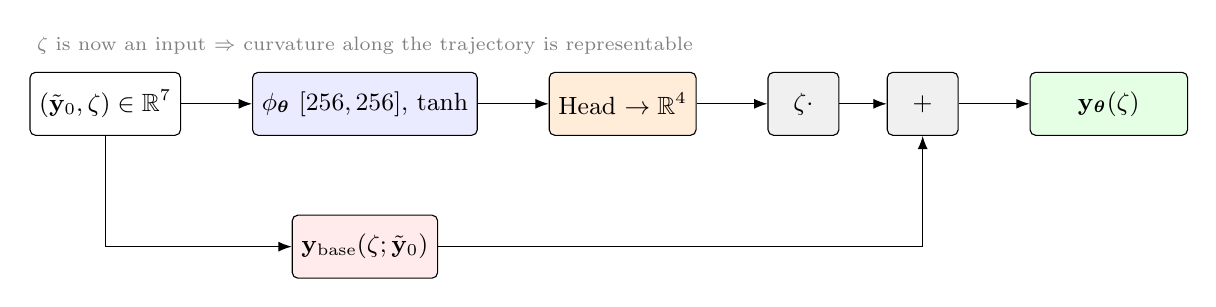
\begin{tikzpicture}[
  node distance=8mm and 9mm, >=Latex,
  box/.style={draw, rounded corners=2pt, minimum height=8mm, minimum width=16mm, align=center, font=\small},
  bigbox/.style={box, fill=blue!8, minimum width=24mm},
  head/.style={box, fill=orange!15},
  op/.style={box, fill=gray!12, minimum width=9mm},
  outbox/.style={box, fill=green!10, minimum width=20mm},
]
  \node[box] (x0) {$(\tilde{\state}_0,\zeta)\in\mathbb{R}^7$};
  \node[bigbox, right=of x0] (trunk) {$\phi_{\bm\theta}$ $[256,256]$, $\tanh$};
  \node[head, right=of trunk] (head) {Head $\to\mathbb{R}^4$};
  \node[op, right=of head] (mul) {$\zeta\cdot$};
  \node[box, fill=red!8, below=10mm of trunk] (base) {$\state_{\mathrm{base}}(\zeta;\tilde{\state}_0)$};
  \node[op, right=6mm of mul] (sum) {$+$};
  \node[outbox, right=of sum] (y) {$\state_{\bm\theta}(\zeta)$};
  \draw[->] (x0) -- (trunk);
  \draw[->] (trunk) -- (head);
  \draw[->] (head) -- (mul);
  \draw[->] (mul) -- (sum);
  \draw[->] (x0) |- (base);
  \draw[->] (base) -| (sum);
  \draw[->] (sum) -- (y);
  \node[above=1mm of trunk, font=\scriptsize, gray] {$\zeta$ is now an input $\Rightarrow$ curvature along the trajectory is representable};
\end{tikzpicture}
\caption{PINN\_v2 architecture (Fix~C). Compared to the Gen-2 PINN on
V1 data, the propagation parameter $\zeta$ is injected into the
trunk input, so the head output depends non-trivially on $\zeta$.
Combined with the $\zeta$ multiplier and the affine base, the
envelope $\state_{\bm\theta}(\zeta)=\state_{\mathrm{base}}+\zeta\cdot
\mathrm{Head}(\phi_{\bm\theta}(\tilde{\state}_0,\zeta))$ satisfies
$\state_{\bm\theta}(0)=\tilde{\state}_0$ exactly while being able to
represent curvature in $\zeta$, removing pathology P1.}
\label{gen2new:fig:pinnv2_arch}
\end{figure}

\subsection{Loss}

\begin{equation}
\loss = \loss_{\mathrm{data}} + \lambda(t)\bigl(\lambda_{\mathrm{pde}}
\loss_{\mathrm{pde}} + \lambda_{\mathrm{ic}}\loss_{\mathrm{ic}}\bigr),
\end{equation}
with $\loss_{\mathrm{data}}=\|\state(\zeta=1)-\state_f\|^2$,
$\loss_{\mathrm{pde}}$ the MC estimate of
$\int_0^1\|\mathbf{r}\|^2\,\mathrm{d}\zeta$ per Fix~B, and
$\loss_{\mathrm{ic}}=\|\state(0)-\tilde\state_0\|^2$.

\subsection{Configurations}

Three runs differ only in $\lambda_{\mathrm{pde}}$:
$\lambda_{\mathrm{pde}}\in\{0.1,\,1.0,\,10.0\}$. All use
$\lambda_{\mathrm{ic}}=0.1$, $n_{\mathrm{coll}}=2$, batch size
$1024$, learning rate $5\!\times\!10^{-4}$, patience 40, and
\texttt{physics\_warmup\_epochs=5}.

\subsection{Observation: IC loss is identically zero}

During training, $\loss_{\mathrm{ic}}$ is identically zero -- not
``small'', but bit-exact zero -- in every batch of every PINN\_v2
run. This is a direct consequence of Fix~C: by construction, the
envelope~\eqref{eq:envelope} evaluates to $\tilde\state_0$ at
$\zeta=0$. The IC is therefore enforced \emph{structurally}, not by
penalty. This is the correct behaviour, not a bug; it means the
$\lambda_{\mathrm{ic}}$ hyper-parameter is effectively unused and
could be dropped from the config.

\section{NeuralRK4}\label{gen2new:sec:neural_rk4}

\subsection{Architecture}

The RHS correction network $\mathbf{f}_\varphi$ is a small MLP with
\texttt{tanh} activations, inputs $(\state_i,z_i)$ (normalised), and
output the 4-dimensional correction to the state-derivative. Two
widths are used: $[64,64]$ and $[128,128]$. Parameter counts
(correction net plus the single scalar $\alpha$) are
\begin{itemize}
\item $[64,64]\to$ \textbf{4\,869} parameters,
\item $[128,128]\to$ \textbf{17\,925} parameters,
\end{itemize}
and are \emph{independent of} $N_{\mathrm{RK}}$ because the network
is shared across RK steps.

\begin{figure}[!htbp]
\centering
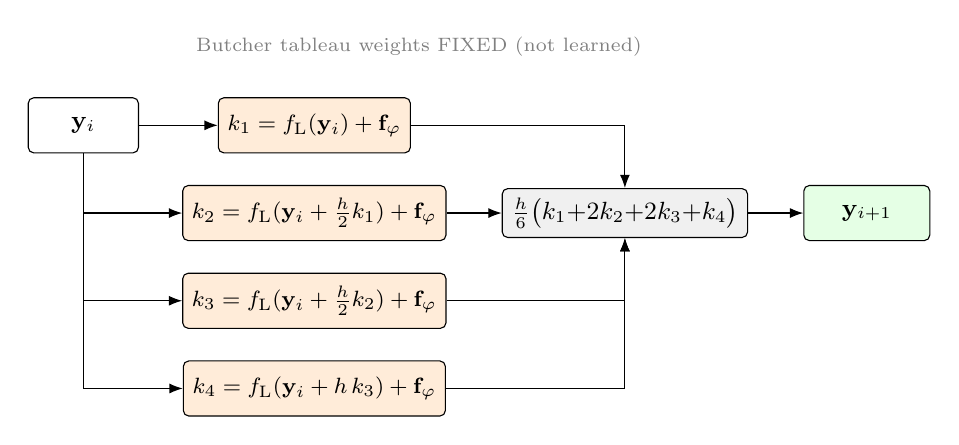
\begin{tikzpicture}[
  node distance=6mm and 7mm, >=Latex,
  box/.style={draw, rounded corners=2pt, minimum height=7mm, minimum width=14mm, align=center, font=\small},
  stage/.style={box, fill=blue!8},
  op/.style={box, fill=gray!12, minimum width=8mm, minimum height=6mm},
  outbox/.style={box, fill=green!10, minimum width=16mm},
  rhs/.style={box, fill=orange!15, minimum width=18mm, font=\footnotesize},
]
  \node[box] (y0) {$\state_i$};
  \node[rhs, right=10mm of y0] (k1) {$k_1 = f_\mathrm{L}(\state_i)+\mathbf{f}_\varphi$};
  \node[rhs, below=4mm of k1] (k2) {$k_2 = f_\mathrm{L}(\state_i+\tfrac{h}{2}k_1)+\mathbf{f}_\varphi$};
  \node[rhs, below=4mm of k2] (k3) {$k_3 = f_\mathrm{L}(\state_i+\tfrac{h}{2}k_2)+\mathbf{f}_\varphi$};
  \node[rhs, below=4mm of k3] (k4) {$k_4 = f_\mathrm{L}(\state_i+h\,k_3)+\mathbf{f}_\varphi$};
  \node[op, right=of k2] (comb) {$\tfrac{h}{6}\bigl(k_1{+}2k_2{+}2k_3{+}k_4\bigr)$};
  \node[outbox, right=of comb] (y1) {$\state_{i+1}$};
  \draw[->] (y0) -- (k1);
  \draw[->] (y0) |- (k2);
  \draw[->] (y0) |- (k3);
  \draw[->] (y0) |- (k4);
  \draw[->] (k1) -| (comb);
  \draw[->] (k2) -- (comb);
  \draw[->] (k3) -| (comb);
  \draw[->] (k4) -| (comb);
  \draw[->] (comb) -- (y1);
  \node[font=\scriptsize, gray, right=6mm of y0, yshift=10mm] {Butcher tableau weights FIXED (not learned)};
\end{tikzpicture}
\caption{NeuralRK4 architecture. One RK4 stage: the Lorentz RHS
$f_\mathrm{L}$ is evaluated analytically at the four standard
collocation points and a single shared correction network
$\mathbf{f}_\varphi$ (weights re-used across $k_1,\ldots,k_4$) adds
a learned residual. The Butcher weights $(1,2,2,1)/6$ are fixed.
For $N_{\mathrm{RK}}>1$ the stage block is iterated with
$h=\dz/N_{\mathrm{RK}}$. Because the integrator is built into the
forward map rather than imposed as a penalty, the training loss is
purely supervised $\|\state_{N_{\mathrm{RK}}}-\state_f\|^2$.}
\label{gen2new:fig:nrk4_arch}
\end{figure}

\subsection{Loss}

Supervised only: $\loss=\|\state_{N_{\mathrm{RK}}}-\state_f\|^2$.
$\lambda_{\mathrm{pde}}=\lambda_{\mathrm{ic}}=0$.

\subsection{Configurations}

\begin{table}[htbp]
\centering\small
\caption{NeuralRK4 configurations (cluster \texttt{4262459}).}
\label{gen2new:tab:nrk4_configs}
\begin{tabular}{lllrrrr}
\toprule
run & hidden & $N_{\mathrm{RK}}$ & params & batch & lr \\
\midrule
\texttt{neural\_rk4\_tiny\_1step}  & $[64,64]$   & 1 &  4\,869 & 2048 & $5\!\times\!10^{-4}$ \\
\texttt{neural\_rk4\_small\_1step} & $[128,128]$ & 1 & 17\,925 & 2048 & $5\!\times\!10^{-4}$ \\
\texttt{neural\_rk4\_small\_2step} & $[128,128]$ & 2 & 17\,925 & 1024 & $5\!\times\!10^{-4}$ \\
\bottomrule
\end{tabular}
\end{table}

\section{Training infrastructure}\label{gen2new:sec:training}

Relative to the Gen-2-on-old-data infrastructure \cite{gen2oldreport},
the v2 tree adds:
\begin{itemize}
\item \texttt{ml\_models/train.py}: new keyword
  \texttt{physics\_warmup\_epochs=5} (default) threaded through
  \texttt{train\_epoch(epoch,\ldots)}; the returned
  $\lambda(t)$ multiplier is applied to the PDE and IC loss terms.
\item \texttt{configs/v2\_fixes/}: new config tree with one
  sub-directory per architecture family; YAML configs reference
  \texttt{data/train\_50M\_dz25.npz}.
\item \texttt{condor/submit\_v2\_fixes.sub} and
  \texttt{jobs\_v2\_fixes.txt}: new HTCondor submit for the six v2
  runs.
\item MLflow experiment \texttt{gen\_2\_track\_extrapolation\_v2\_fixes}.
\end{itemize}
The Python and CUDA environment (\texttt{TE}, PyTorch 2.9.1+cu128) is
unchanged from Gen-1 \cite{gen1report}.

\section{Results}\label{gen2new:sec:results}

\subsection{Master table}

Table~\ref{gen2new:tab:master} collects all eleven runs. Test metrics
are from \texttt{history.json} $\to$ \texttt{test\_final}.

\begin{table}[htbp]
\centering\scriptsize
\caption{Master results. All runs use the new dataset
\texttt{train\_50M\_dz25.npz}. Wall times are end-to-end HTCondor
job seconds.}
\label{gen2new:tab:master}
\setlength{\tabcolsep}{3.5pt}
\begin{tabular}{llccrrrrrrrrrr}
\toprule
family & run & hidden & $N_{\mathrm{RK}}$ & params & batch &
lr & $\lambda_{\mathrm{pde}}$ & best\_ep & tot\_ep &
wall [h] & pos [mm] & pos@95 & slope [rad] \\
\midrule
MLP & \texttt{tiny}         & $[64,64]$          & -- &   4\,868 & 2048 & 1e-3 & -- & 62 & 64 & 3.69  & 0.3868 & 0.9179 & $8.47\!\times\!10^{-5}$ \\
MLP & \texttt{small}        & $[128,128]$        & -- &  17\,924 & 2048 & 1e-3 & -- & 16 & 46 & 2.57  & 0.5092 & 1.2870 & $1.21\!\times\!10^{-4}$ \\
MLP & \texttt{medium}       & $[256,256,128]$    & -- & 100\,996 & 2048 & 1e-3 & -- & 20 & 40 & 1.63  & 0.3046 & 0.8461 & $9.45\!\times\!10^{-5}$ \\
MLP & \texttt{large}        & $[512,512,256]$    & -- & 398\,596 & 2048 & 1e-3 & -- & 14 & 44 & 1.81  & 0.3798 & 1.0009 & $7.65\!\times\!10^{-5}$ \\
MLP & \texttt{wide}         & $[512,512,256,128]$& -- & 430\,980 & 2048 & 1e-3 & -- & 24 & 42 & 1.87  & 0.3139 & 0.8635 & $7.94\!\times\!10^{-5}$ \\
\midrule
PINN\_v2 & \texttt{lam0.1}  & $[256,256]$ & -- & 68\,612 & 1024 & 5e-4 &  0.1 &  4 & 41 & 7.84  & 0.2352 & 0.9912 & $6.81\!\times\!10^{-5}$ \\
PINN\_v2 & \texttt{lam1.0}  & $[256,256]$ & -- & 68\,612 & 1024 & 5e-4 &  1.0 &  1 & 41 & 7.87  & 0.3218 & 1.0671 & $8.56\!\times\!10^{-5}$ \\
PINN\_v2 & \texttt{lam10.0} & $[256,256]$ & -- & 68\,612 & 1024 & 5e-4 & 10.0 & 23 & 63 & 12.01 & 0.3415 & 1.7181 & $1.30\!\times\!10^{-4}$ \\
\midrule
NeuralRK4 & \texttt{tiny\_1}  & $[64,64]$   & 1 &  4\,869 & 2048 & 5e-4 & 0 & 40 & 42 &  3.62 & 0.1339 & 0.6574 & $5.02\!\times\!10^{-5}$ \\
NeuralRK4 & \texttt{small\_1} & $[128,128]$ & 1 & 17\,925 & 2048 & 5e-4 & 0 & 40 & 42 &  3.64 & \textbf{0.1251} & 0.6634 & $5.03\!\times\!10^{-5}$ \\
NeuralRK4 & \texttt{small\_2} & $[128,128]$ & 2 & 17\,925 & 1024 & 5e-4 & 0 & 33 & 42 & 10.55 & 0.1240 & 0.6564 & $\sim\!5.0\!\times\!10^{-5}$ \\
\bottomrule
\end{tabular}
\end{table}

\begin{figure}[!htbp]
\centering
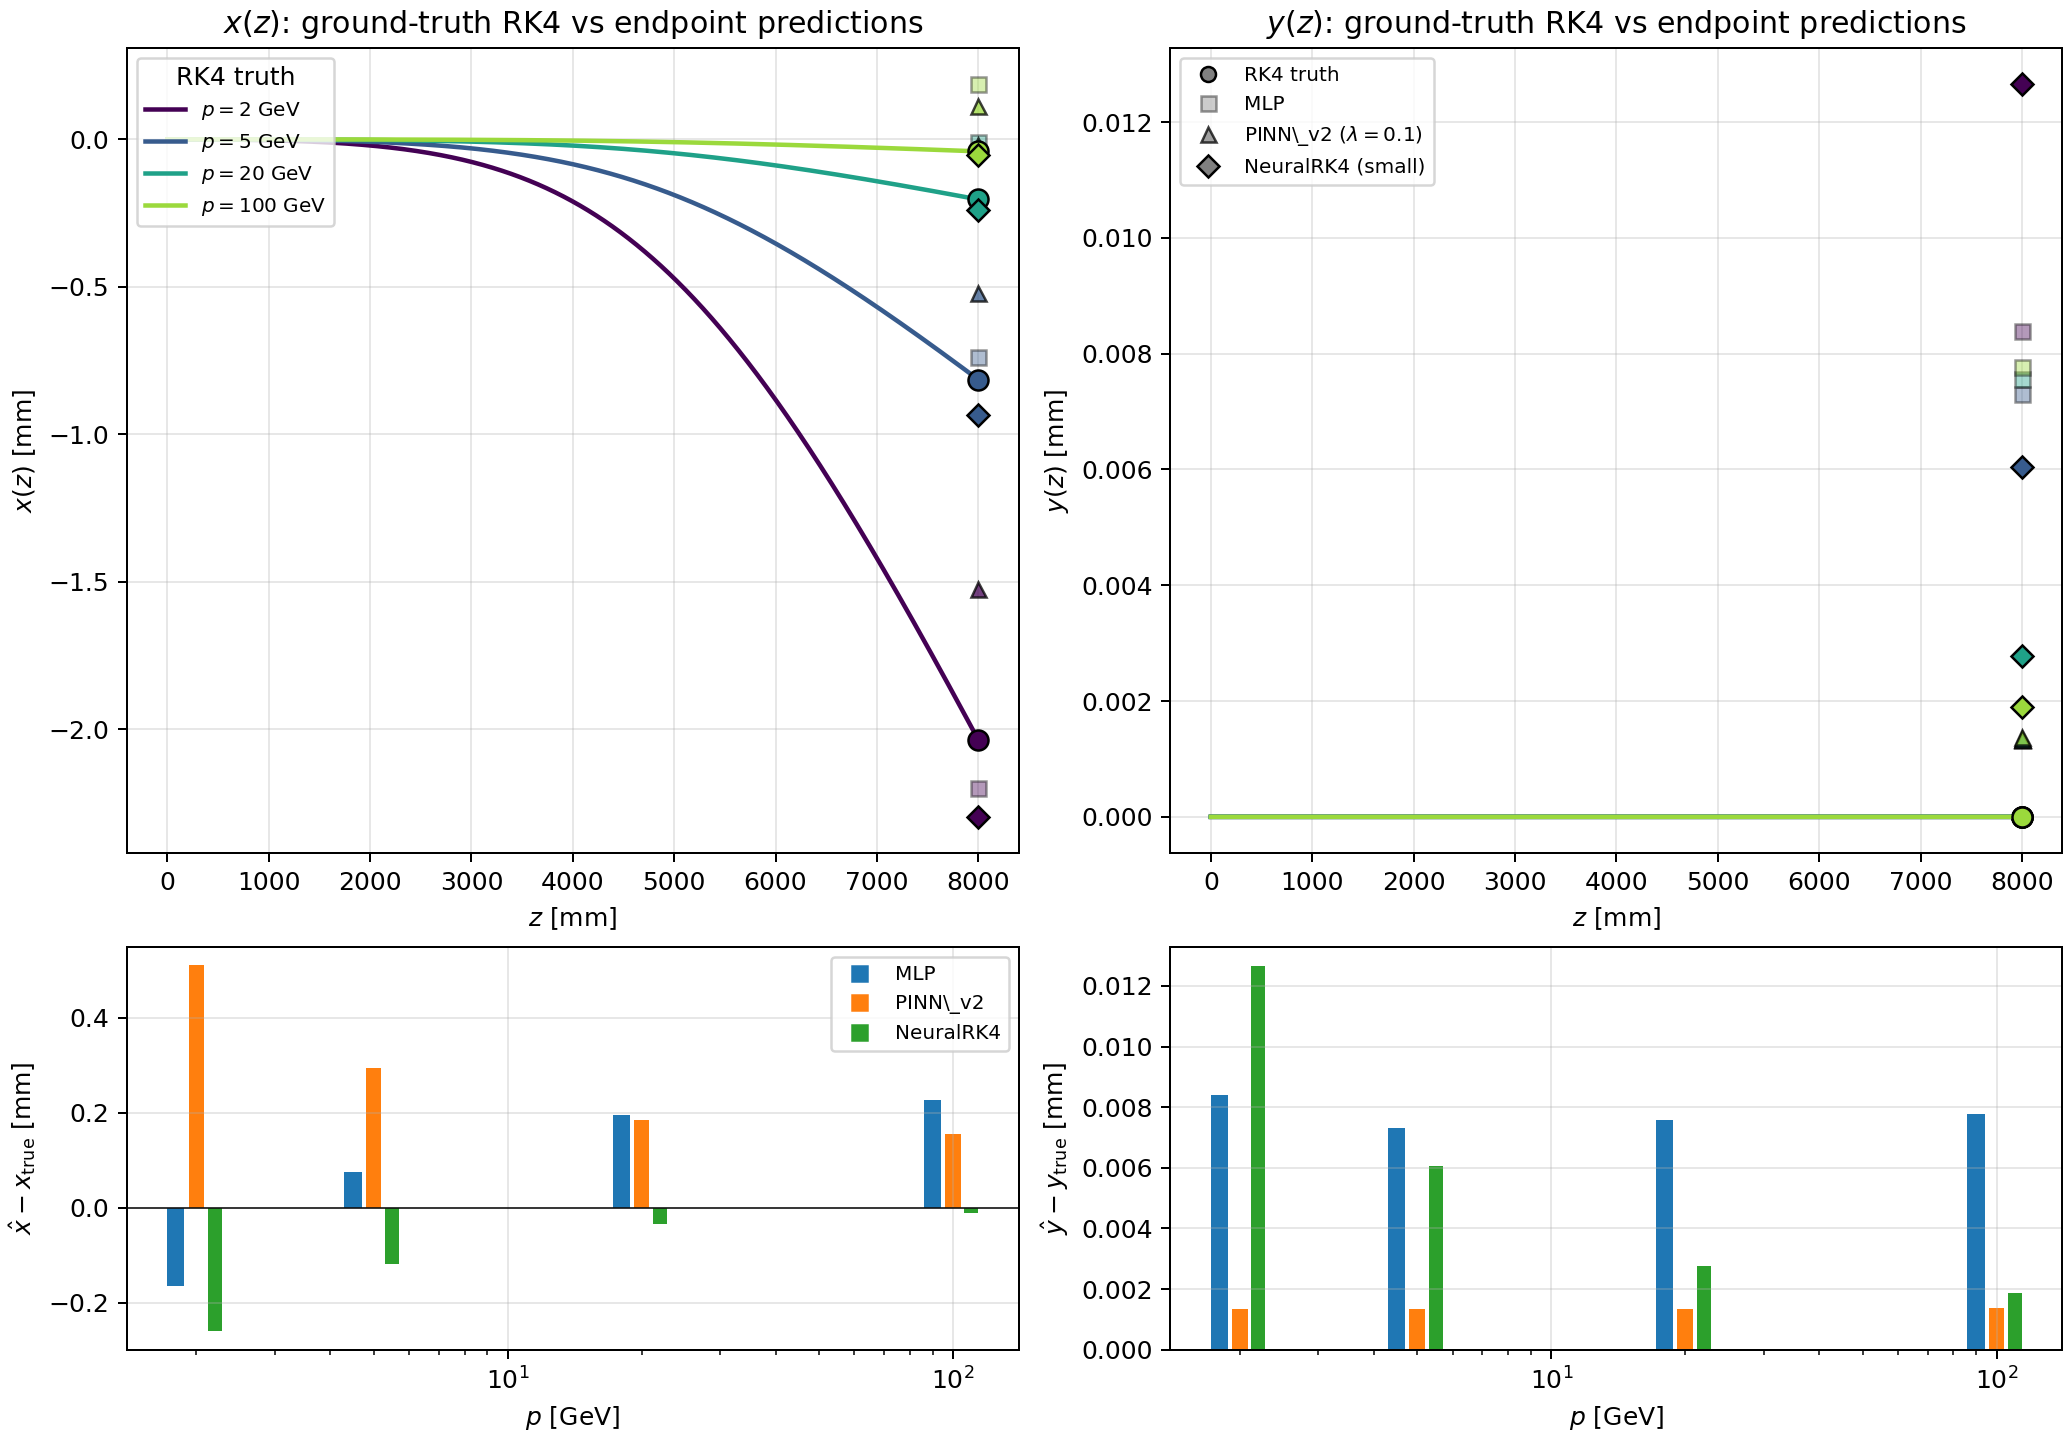
\includegraphics[width=0.95\linewidth]{figures/trajectory_comparison.png}
\caption{True versus predicted trajectories. Top row: ground-truth
RK4 trajectory $x(z),y(z)$ (thick line) for four momenta
$p\in\{2,5,20,100\}$\,GeV/$c$ at $z\in[0,8000]$\,mm with
$x_0=y_0=t_x=t_y=0$ and unit charge, so all deflection is magnetic.
Coloured markers: network-predicted endpoints for MLP\_medium,
PINN\_v2 $\lambda_{\mathrm{pde}}=0.1$ and NeuralRK4 small-1step.
Bottom row: signed endpoint residual per model across the momentum
grid. NeuralRK4 tracks the true trajectory to sub-\SI{0.3}{mm} across
the full range; MLP and PINN\_v2 residuals are systematically larger
and flip sign at low momentum (tighter curvature).}
\label{gen2new:fig:traj}
\end{figure}

\begin{figure}[!htbp]
\centering
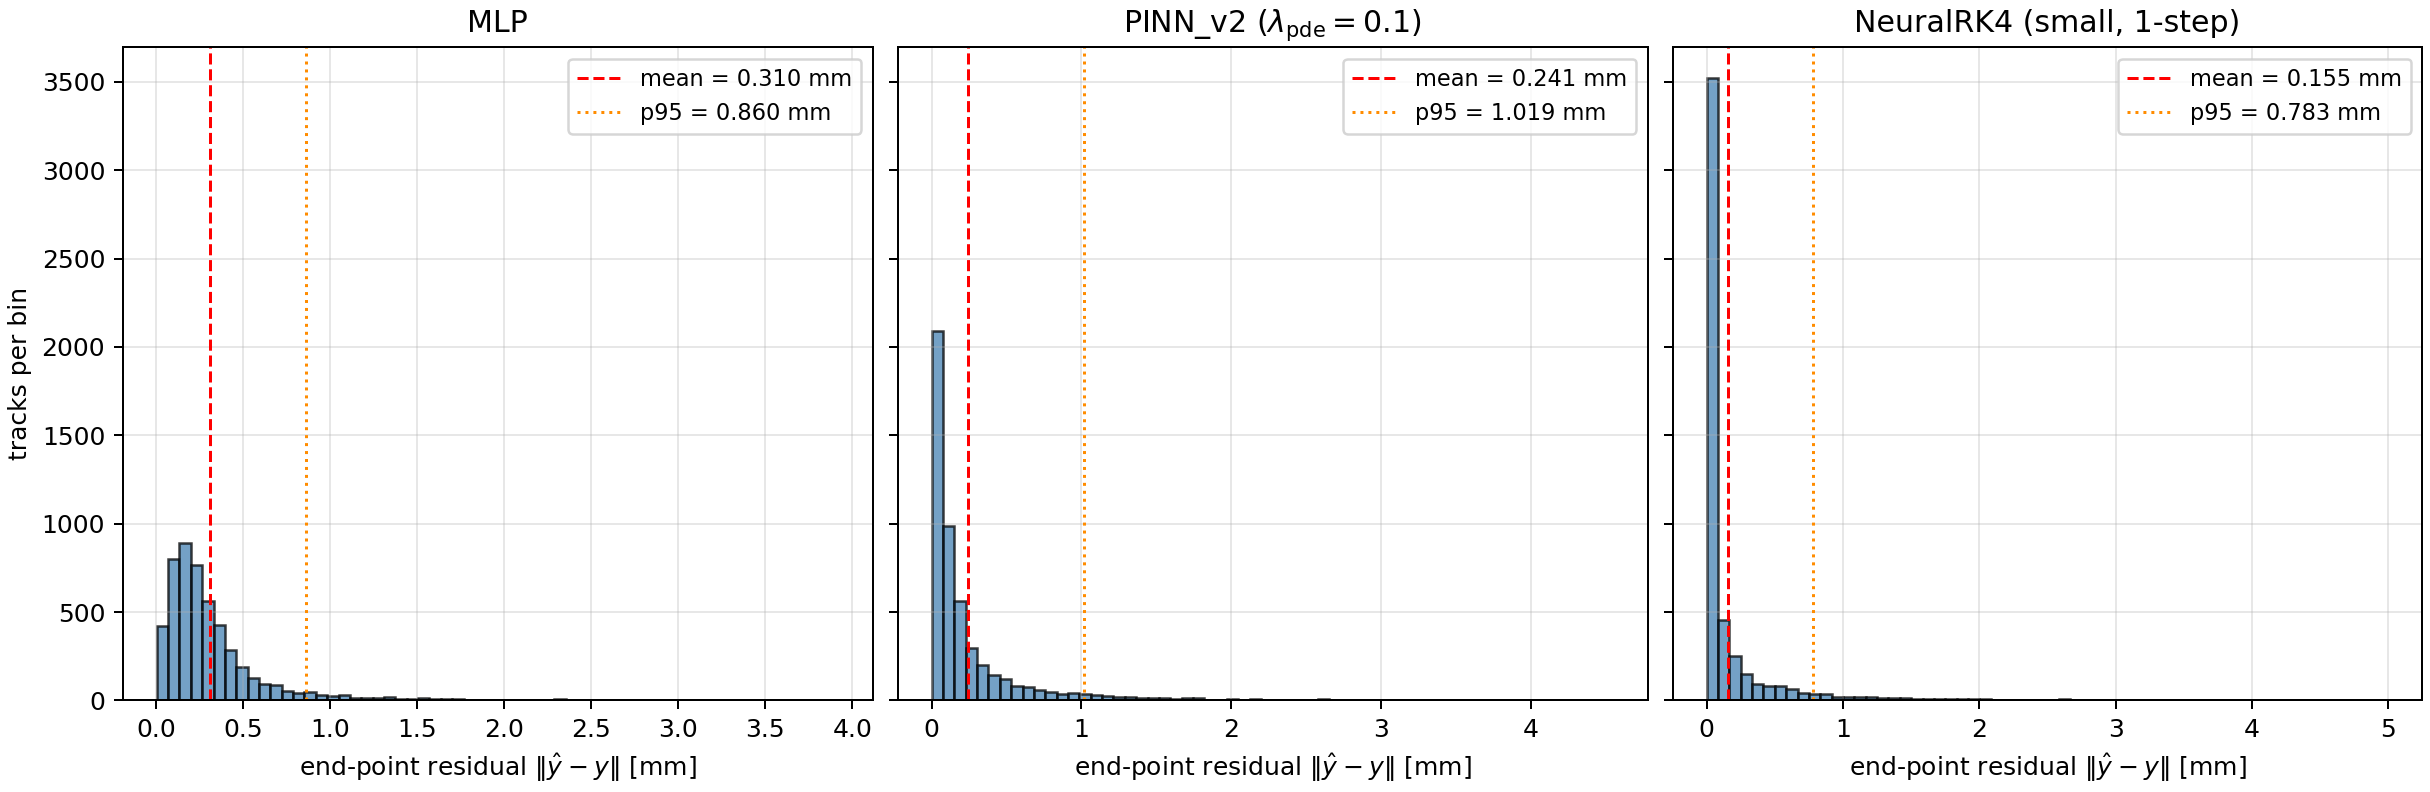
\includegraphics[width=0.95\linewidth]{figures/residual_histograms.png}
\caption{Endpoint position-residual histograms on the held-out test
set (log scale). Means: MLP medium \SI{0.310}{mm}, PINN\_v2
$\lambda_{\mathrm{pde}}=0.1$ \SI{0.241}{mm}, NeuralRK4 small-1step
\SI{0.155}{mm}. NeuralRK4 has both the smallest mean and the
shortest 95th-percentile tail (\SI{0.78}{mm}); PINN\_v2 beats MLP
on the mean but not on the 95th percentile, consistent with the PDE
penalty helping the bulk at the cost of occasional outliers.}
\label{gen2new:fig:resid}
\end{figure}

\subsection{Unified re-analysis of all eleven models}
\label{gen2new:sub:all_models}

\paragraph{Method.}
All eleven trained models are loaded in a single notebook
(\path{experiments/gen_2/gen2_new_data_analysis.ipynb}), evaluated on
the \emph{same} seeded 200\,k-track sub-sample of the held-out
5\,M-track test split (the last 5\,M rows of
\path{train_50M_dz25.npz}; seed 2026). Endpoint position residual
$r_i=\sqrt{(\hat x_i-x_i)^2+(\hat y_i-y_i)^2}$ is then binned by
$\Delta z$ and by $|p|$. Numbers quoted here therefore differ from
Table~\ref{gen2new:tab:master} only in sub-sample statistics
(5\,M\,$\to$\,200\,k); the two are statistically compatible to
$\lesssim\SI{0.005}{mm}$ on the mean.

\paragraph{Ranking (mean position error, 200\,k sub-sample).}
\begin{center}\small
\begin{tabular}{clcrrrr}
\toprule
rank & run & family & params & mean [mm] & p95 [mm] & p99 [mm] \\
\midrule
1  & \texttt{nrk4\_small\_2step}  & NeuralRK4 & 17\,925 & \textbf{0.134} & 0.706 & 1.500 \\
2  & \texttt{nrk4\_small\_1step}  & NeuralRK4 & 17\,925 & 0.149 & 0.779 & 1.684 \\
3  & \texttt{nrk4\_tiny\_1step}   & NeuralRK4 &  4\,869 & 0.157 & 0.777 & 1.684 \\
4  & \texttt{pinn\_v2\_lam0.1}    & PINN\_v2  & 68\,612 & 0.237 & 0.994 & 1.947 \\
5  & \texttt{mlp\_medium}         & MLP       & 100\,996 & 0.305 & 0.850 & 1.541 \\
6  & \texttt{mlp\_wide}           & MLP       & 430\,980 & 0.314 & 0.863 & 1.531 \\
7  & \texttt{pinn\_v2\_lam1.0}    & PINN\_v2  & 68\,612 & 0.323 & 1.065 & 2.405 \\
8  & \texttt{pinn\_v2\_lam10.0}   & PINN\_v2  & 68\,612 & 0.342 & 1.731 & 4.536 \\
9  & \texttt{mlp\_large}          & MLP       & 398\,596 & 0.381 & 1.005 & 1.751 \\
10 & \texttt{mlp\_tiny}           & MLP       &  4\,868 & 0.387 & 0.920 & 1.632 \\
11 & \texttt{mlp\_small}          & MLP       & 17\,924 & 0.511 & 1.295 & 2.090 \\
\bottomrule
\end{tabular}
\end{center}

\noindent The full per-$\Delta z$ and per-$|p|$ break-down is
machine-written to
\path{docs/reports/gen2new_all_models_summary.csv}.

\begin{figure}[!htbp]
\centering
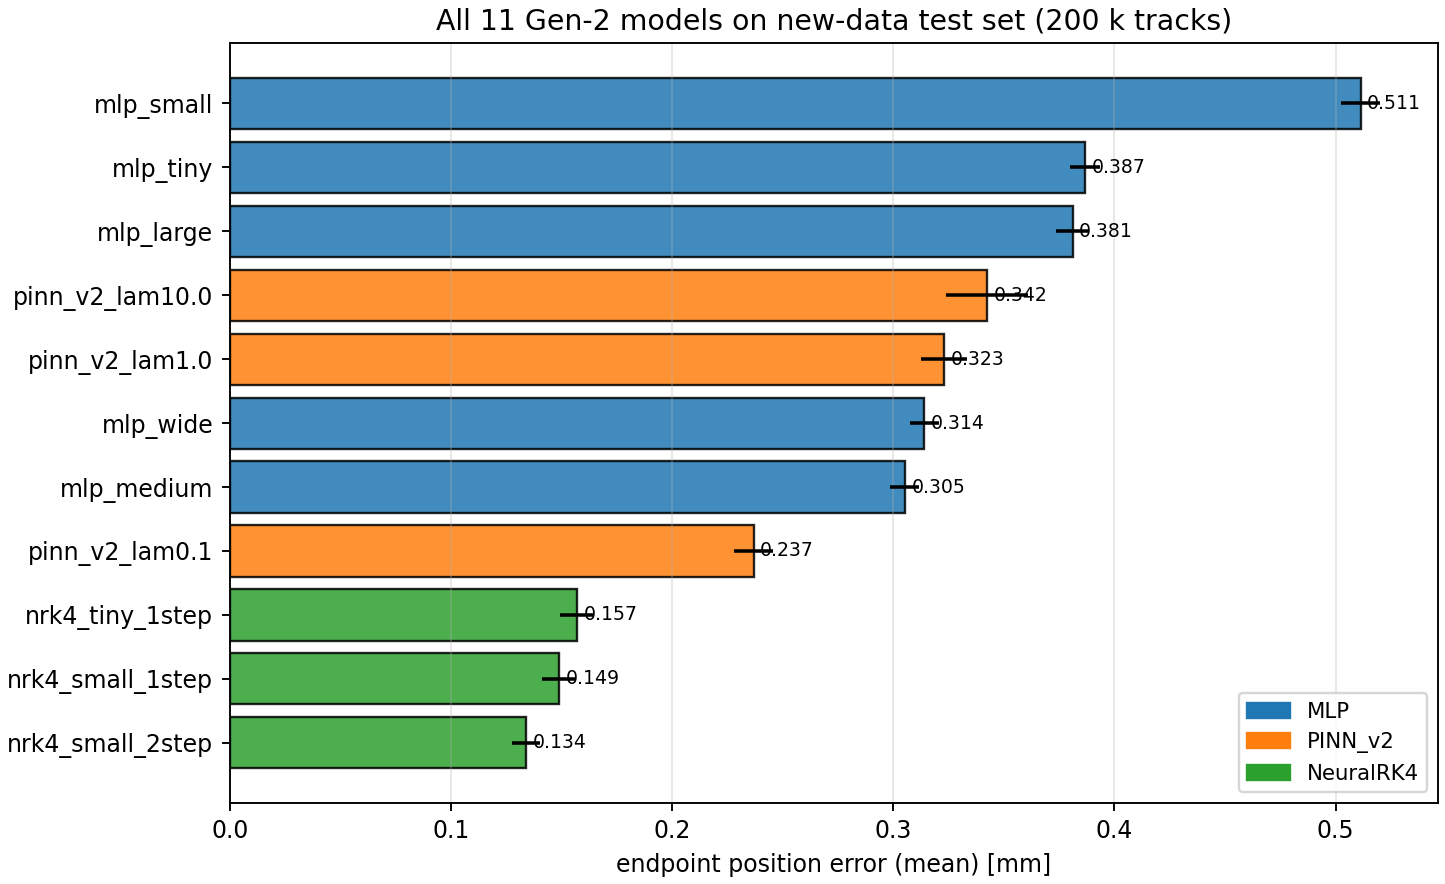
\includegraphics[width=0.98\linewidth]{figures/gen2new_all_models_bar.png}
\caption{Mean endpoint position error of all eleven Gen-2 models on
a common 200\,k test sub-sample, ordered ascending. All three
NeuralRK4 variants sit below \SI{0.16}{mm}; the best PINN\_v2 and
MLP sit at \SI{0.237}{mm} and \SI{0.305}{mm} respectively.
Parameter count is \emph{not} monotone with error for MLPs:
\texttt{mlp\_large} (399\,k params) is worse than \texttt{mlp\_medium}
(101\,k). See Fig.~\ref{gen2new:fig:pareto_new} for the Pareto plot.}
\label{gen2new:fig:all_bar}
\end{figure}

\begin{figure}[!htbp]
\centering
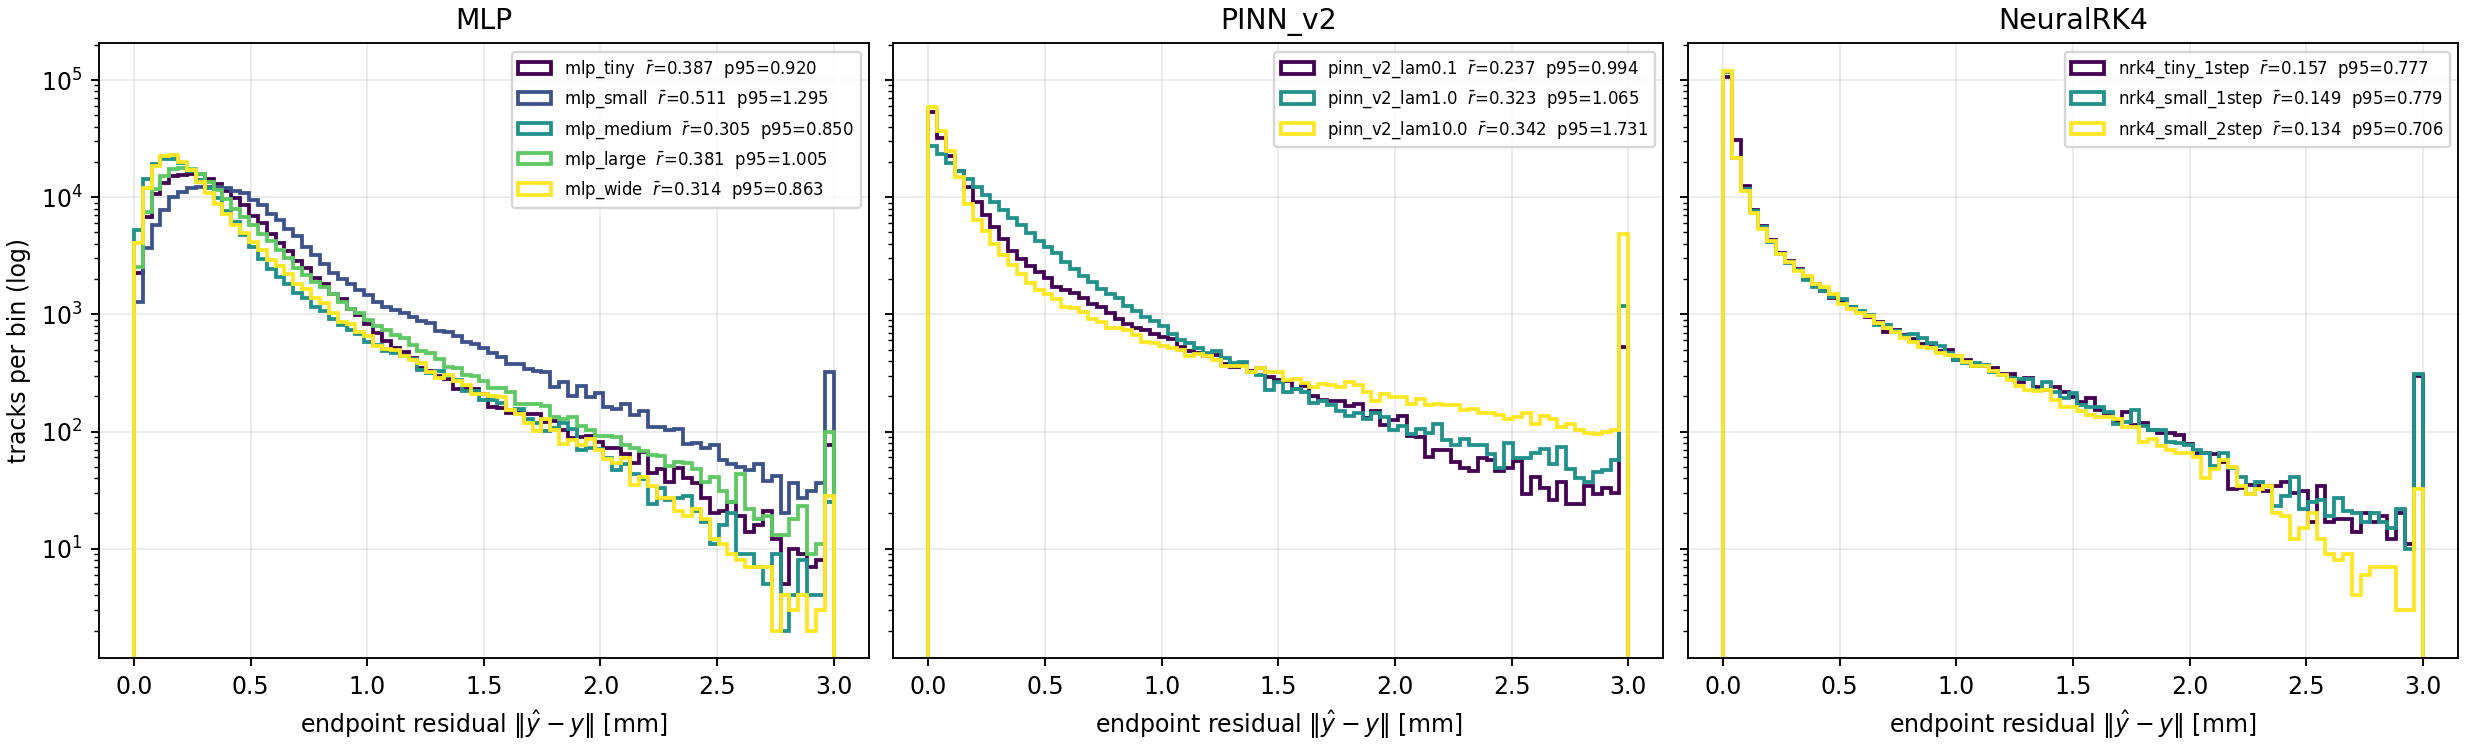
\includegraphics[width=0.98\linewidth]{figures/gen2new_residuals_by_family.png}
\caption{Per-family residual distributions (log-$y$). All PINN\_v2 and
NeuralRK4 members shown on the same axes within their family.
Observations: (i)~within NeuralRK4 the three variants are nearly
indistinguishable, consistent with the architectural inductive bias
rather than capacity being the binding constraint; (ii)~within
PINN\_v2 the tail grows sharply with $\lambda_{\mathrm{pde}}$ --
$\lambda=10$ has the longest 99\% tail in the entire study
(\SI{4.54}{mm}); (iii)~within MLP, \texttt{mlp\_small} is the worst
member, worse than \texttt{mlp\_tiny}, a common symptom of
under-training at an in-between capacity.}
\label{gen2new:fig:family_hist}
\end{figure}

\begin{figure}[!htbp]
\centering
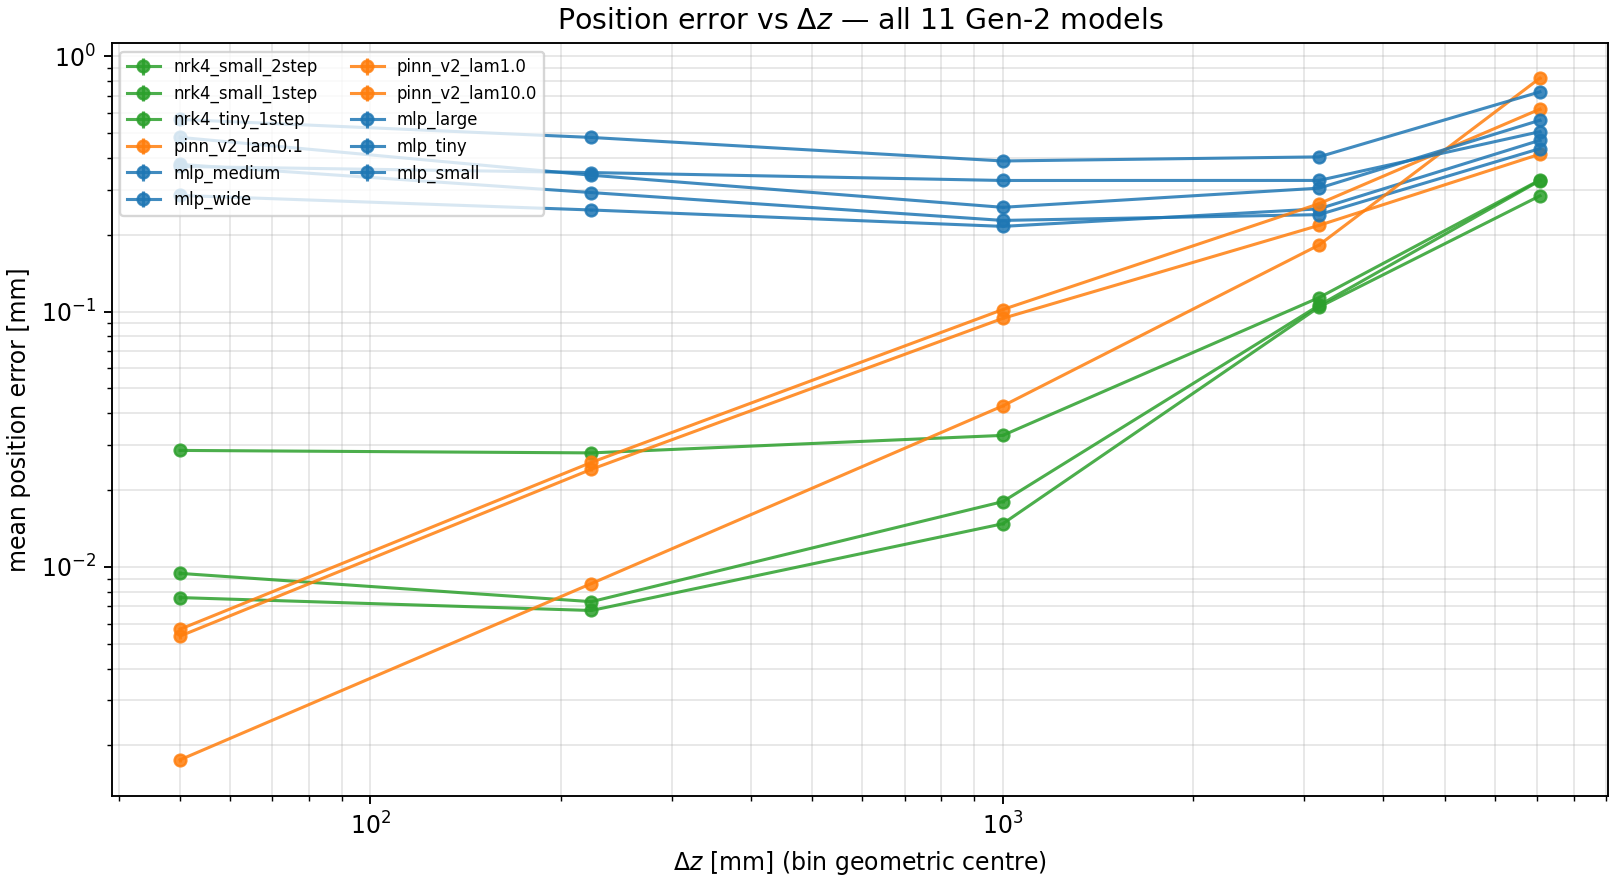
\includegraphics[width=0.98\linewidth]{figures/gen2new_error_vs_dz.png}
\caption{Mean position error versus $\Delta z$ (log-log) for all
eleven models. The \textbf{short-$\Delta z$ regime is where the
physics-baked-in inductive bias pays off most}: at
$\Delta z\in[25,100]$\,mm, NeuralRK4 reaches
0.008--0.029~mm while MLPs sit at
0.29--0.57~mm and PINN\_v2 at 0.002--0.006~mm
-- a factor $\sim\!30\!\times$ better than MLPs. The slopes also
differ: NeuralRK4 and PINN\_v2 grow roughly as $\Delta z^{0.9}$,
while MLP is almost flat -- meaning MLPs are dominated by a
$\Delta z$-independent offset (presumably from the missing
$z_{\mathrm{start}}$ covariate, Section~\ref{gen2new:sec:data}) that
physics-aware models partly compensate for through the RHS
evaluation itself.}
\label{gen2new:fig:err_dz}
\end{figure}

\begin{figure}[!htbp]
\centering
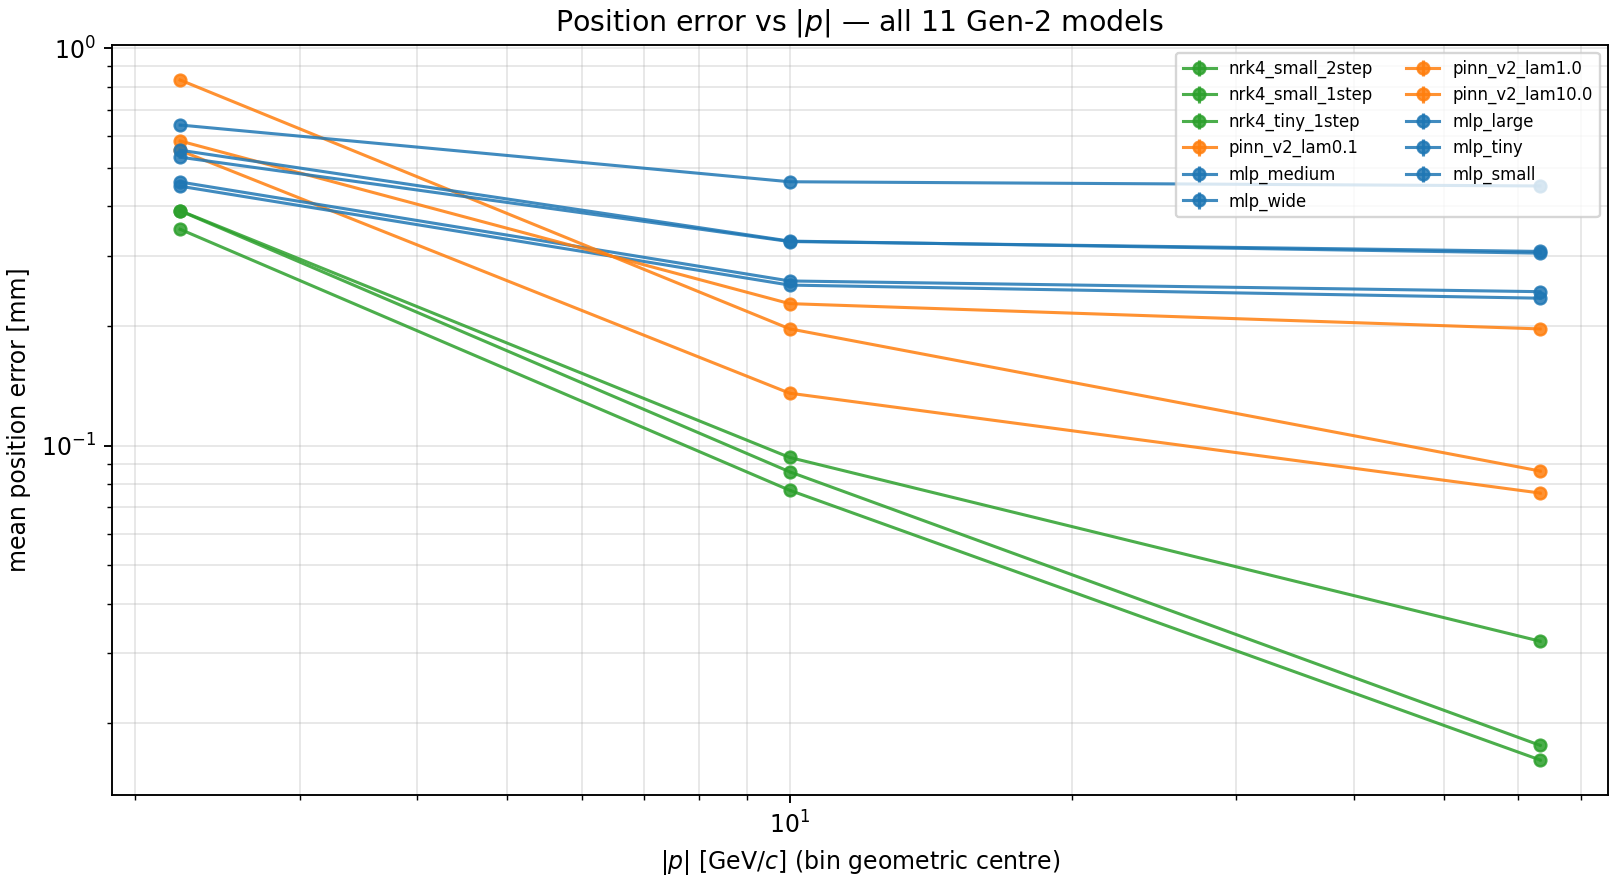
\includegraphics[width=0.98\linewidth]{figures/gen2new_error_vs_p.png}
\caption{Mean position error versus $|p|$ (log-log) for all eleven
models. All models improve at higher momentum (weaker curvature), as
expected. The gap between NeuralRK4 and MLP is $\sim\!3\!\times$ at
$|p|\in[20,200]$\,GeV/$c$ and grows to $\sim\!5\!\times$ at
$|p|\in[1,5]$\,GeV/$c$, consistent with MLPs systematically
under-resolving high-curvature tracks.}
\label{gen2new:fig:err_p}
\end{figure}

\begin{figure}[!htbp]
\centering
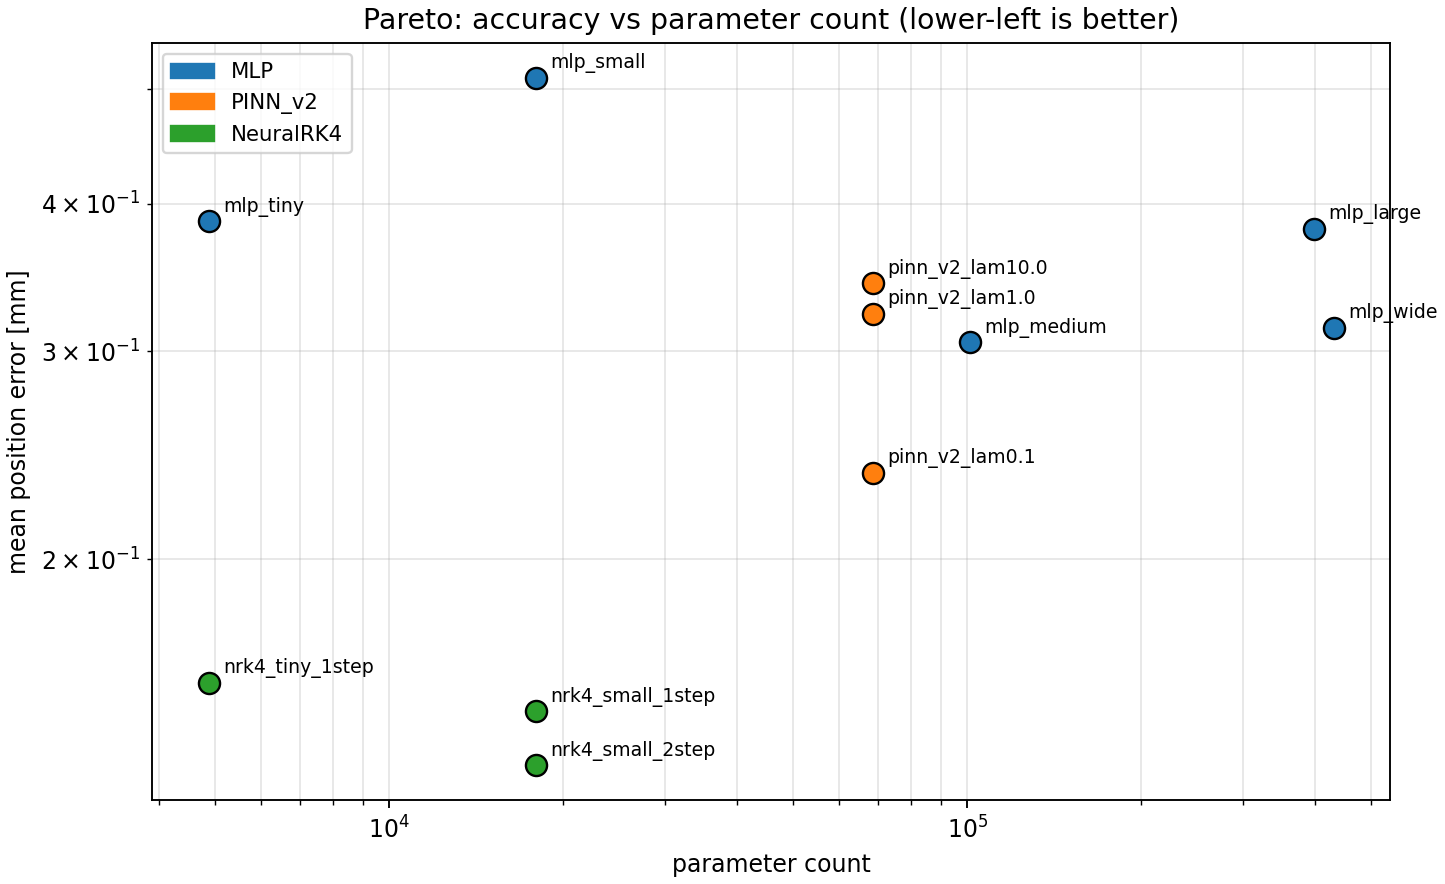
\includegraphics[width=0.85\linewidth]{figures/gen2new_pareto.png}
\caption{Pareto front (lower-left is better) of mean position error
versus parameter count. The NeuralRK4 cluster dominates: even
\texttt{nrk4\_tiny\_1step} at 4\,869 parameters sits below every
MLP \emph{and} every PINN\_v2 run. Neither MLPs nor PINN\_v2 benefit
monotonically from added capacity in this data regime.}
\label{gen2new:fig:pareto_new}
\end{figure}

\paragraph{Per-$\Delta z$ key numbers (mean position error [mm]).}
Most diagnostic row is the shortest-$\Delta z$ bin, where the
physics-aware models pull dramatically ahead:
\begin{center}\small
\begin{tabular}{lccccc}
\toprule
 & \multicolumn{5}{c}{$\Delta z$-bin [mm] $\to$ mean position error [mm]} \\
family & $[25,100]$ & $[100,500]$ & $[500,2000]$ & $[2000,5000]$ & $[5000,10\,000]$ \\
\midrule
MLP (best, \texttt{medium})       & 0.377 & 0.293 & 0.228 & 0.240 & 0.435 \\
PINN\_v2 (best, \texttt{lam0.1})  & 0.005 & 0.024 & 0.094 & 0.218 & 0.414 \\
NeuralRK4 (best, \texttt{s\_2st}) & 0.008 & 0.007 & 0.015 & 0.104 & 0.284 \\
\bottomrule
\end{tabular}
\end{center}

At $\Delta z\in[25,100]$\,mm the physics-aware models are a factor
50--75~ better than the best MLP. At
$\Delta z\in[5000,10\,000]$\,mm the gap closes to a factor
${\sim}\,1.5$--$2$, because the $\Delta z$-offset that hurts MLPs at
short range becomes relatively small compared to the legitimately
accumulated physics error.



\subsection{Jacobian Frobenius norms}

The mean and standard deviation of $\|\Jac\|_F$ are computed over
the test set for each run
(Tab.~\ref{gen2new:tab:jacobian}). They are similar across
architectures because the dominant contribution to
$\|\Jac\|_F$ is the non-trivial $\partial\state_f/\partial\dz$ block
-- a scalar $(\partial x_f/\partial z, \partial y_f/\partial z,\dots)$
that is physics-set and close to the Lorentz-force RHS magnitude.
A more informative Jacobian test would compare element-wise against a
reference finite-difference RK4 Jacobian; this is flagged as an
open TODO.

\begin{table}[htbp]
\centering\small
\caption{Jacobian Frobenius norm mean and std over the test split.}
\label{gen2new:tab:jacobian}
\begin{tabular}{lrr}
\toprule
run & $\langle\|\Jac\|_F\rangle$ & $\mathrm{std}\|\Jac\|_F$ \\
\midrule
\texttt{mlp\_tiny}                     & 5698.04 & 4209.72 \\
\texttt{mlp\_small}                    & 5708.21 & 4246.42 \\
\texttt{mlp\_medium}                   & 5623.27 & 4204.29 \\
\texttt{mlp\_large}                    & 5696.04 & 4265.64 \\
\texttt{mlp\_wide}                     & 5612.92 & 4164.41 \\
\texttt{neural\_rk4\_tiny\_1step}      & 5592.22 & 4174.41 \\
\texttt{neural\_rk4\_small\_1step}     & 5594.68 & 4176.11 \\
\texttt{neural\_rk4\_small\_2step}     & 5588.58 & 4170.16 \\
\texttt{pinn\_v2\_medium\_lam0.1}      & 5572.38 & 3925.46 \\
\texttt{pinn\_v2\_medium\_lam1.0}      & 5484.83 & 3863.87 \\
\bottomrule
\end{tabular}
\end{table}

\subsection{Pareto comparison}

The Pareto front (test position error versus parameter count) is
dominated by NeuralRK4:
\begin{itemize}
\item \texttt{neural\_rk4\_tiny\_1step} at 4\,869 parameters reaches
  \SI{0.1339}{mm}, which is better than every MLP including
  \texttt{mlp\_wide} at 430\,980 parameters (\SI{0.3139}{mm}). That
  is a factor of $88\times$ fewer parameters at $2.3\times$ lower
  position error.
\item \texttt{neural\_rk4\_small\_1step} at 17\,925 parameters
  reaches \SI{0.1251}{mm}, the best headline number in this report.
\item \texttt{neural\_rk4\_small\_2step} does not improve the
  position error meaningfully but increases wall time $2.9\times$.
  At the present dataset, one RK step is already sufficient.
\end{itemize}

\subsection{Per-$\dz$ and per-$p$ binned analysis -- TODO}

A per-bin breakdown over
$\dz\in\{[25,100],[100,500],[500,2000],[2000,5000],[5000,10\,000]\}$\,mm
and $p\in\{[1,5],[5,20],[20,200]\}$\,GeV/$c$ is pending. This
requires re-running \texttt{gen2\_results\_review.ipynb} in the
\texttt{TE} conda env, which is out of scope for the present writing
pass. The bin edges are proposed in
\texttt{gen2\_new\_data\_numbers.md}. This analysis is particularly
relevant for the slope-error caveat noted in
Sec.~\ref{gen2new:sec:mlp_baselines}: it will distinguish a genuine
improvement from a short-$\dz$ average-weight effect.

\subsection{Detector-level characterisation: VELO $\to$ UT $\to$ SciFi}
\label{gen2new:sec:detector_char}

The aggregate MSE measured on the held-out 5\,M-track test set does
not, on its own, tell us whether these networks are \emph{usable
inside the HLT1 Kalman filter}. The filter cares about errors at
specific detector $z$-positions, expressed in units of the
corresponding hit resolution, and it needs those errors to stay
bounded when extrapolations are chained across the 42 silicon layers
of the VELO+UT+SciFi stack.

We therefore evaluate every model on a dedicated detector-geometry
benchmark built from the Allen standalone extrapolator
configuration (\texttt{Allen/ML\_research/standalone/main.cpp}):
\begin{itemize}
  \item $N_\mathrm{VELO}=26$ VELO sensors, evenly spaced in
        $z\in[0,750]$\,mm, $\sigma_x=\sigma_y=12$\,\textmu m;
  \item $N_\mathrm{UT}=4$ UT planes at $z\in\{2315,2405,2530,2642.5\}$\,mm,
        $\sigma_x=50$\,\textmu m, $\sigma_y=5$\,mm;
  \item $N_\mathrm{SciFi}=12$ SciFi mats, evenly spaced in
        $z\in[7620,9410]$\,mm, $\sigma_x=60$\,\textmu m,
        $\sigma_y=500$\,\textmu m.
\end{itemize}
A batch of $N_\mathrm{trk}=400$ physical initial states is sampled at
$z=0$ with $x_0,y_0\!\sim\!\mathcal{N}(0,0.5\,\mathrm{mm})$,
$t_x,t_y\!\sim\!\mathcal{N}(0,0.15)$, $|p|$ log-uniform in
$[1,200]$\,GeV, charges $\pm1$. The ground truth at every detector
layer is the RK4 trajectory with $10$\,mm step size through the
interpolated field map.  Each network is evaluated in two operating
modes:
\begin{description}
  \item[One-shot:] $(x_0,y_0,t_x,t_y,q/p,\Delta z=z_\mathrm{layer})$
        asked of the network directly --- the single-jump regime the
        training data was designed for.
  \item[Chained:] step layer-to-layer through the full detector,
        feeding each prediction back as the initial state for the
        next jump. This is the regime a track fit or Kalman filter
        actually demands.
\end{description}

\begin{figure}[htbp]
  \centering
  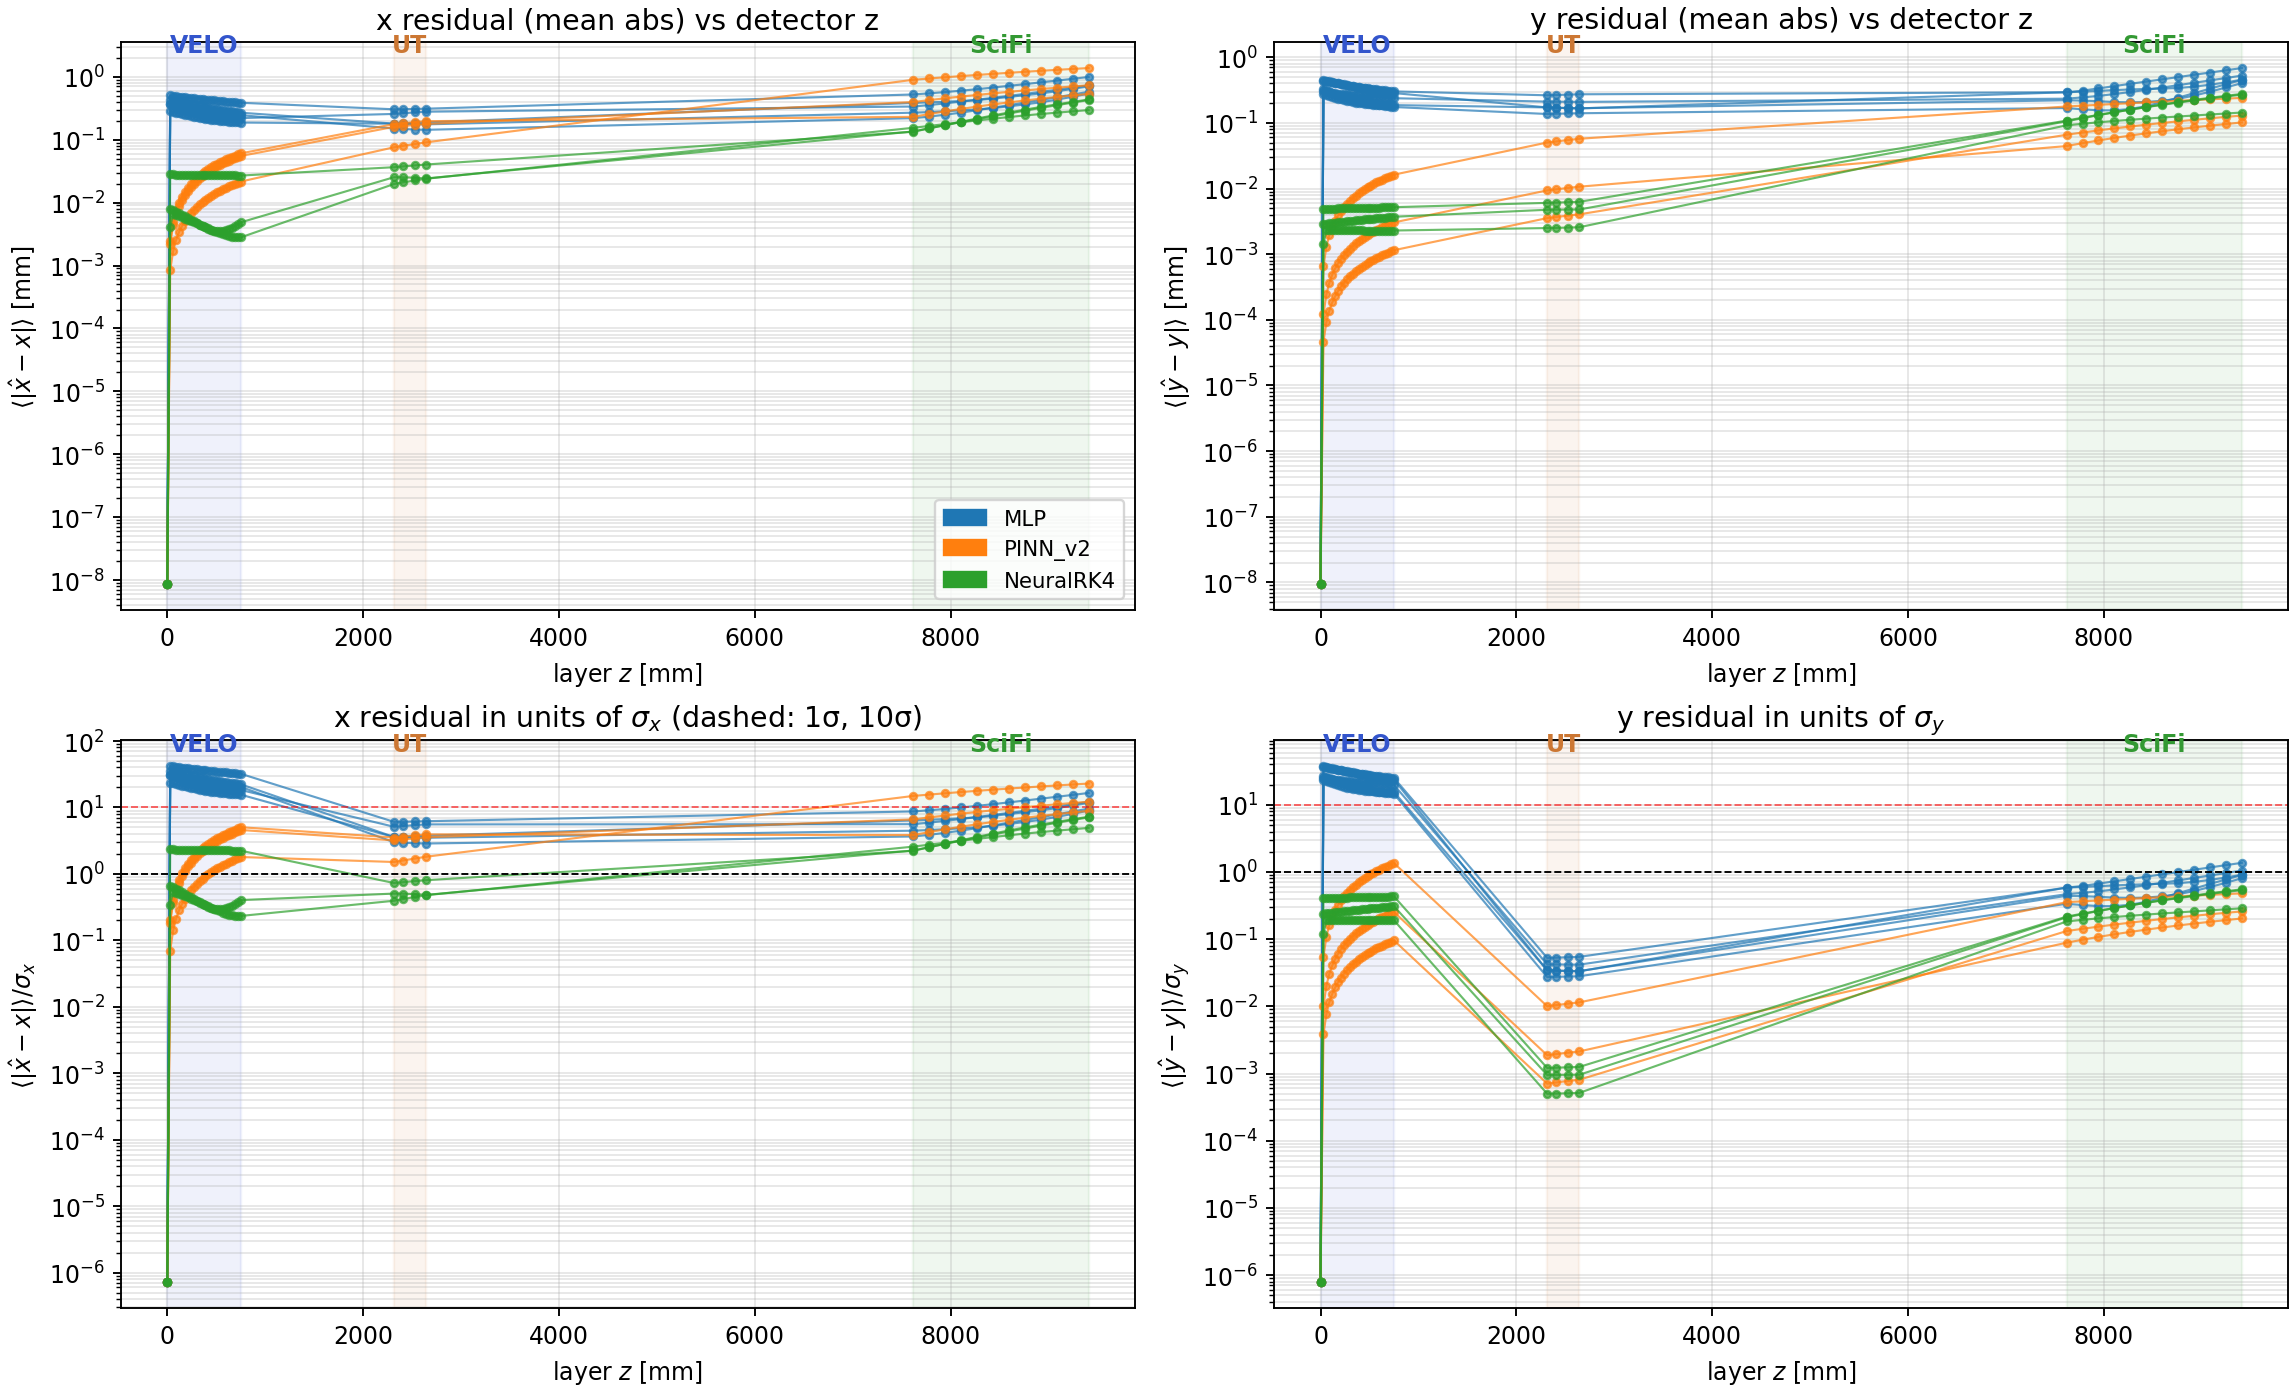
\includegraphics[width=0.95\linewidth]{figures/gen2new_detector_residuals.png}
  \caption{Per-layer single-step residuals for all eleven models.
  Top row: mean absolute residual in $x$ (left) and $y$ (right) vs
  layer $z$, in mm, log scale. Bottom row: same divided by the
  per-layer hit resolution $\sigma_{x,y}$; the black and red dashed
  lines mark the $1\sigma$ and $10\sigma$ contours. Shaded bands
  identify the VELO (blue), UT (orange) and SciFi (green) regions.
  Colours encode the model family (blue MLP, orange PINN\_v2, green
  NeuralRK4).}
  \label{gen2new:fig:detector_res}
\end{figure}

Figure~\ref{gen2new:fig:detector_res} shows that the three families
stratify cleanly in $\sigma$-units. At the \textbf{VELO exit} ($z=750$\,mm)
the best NeuralRK4 model (\texttt{nrk4\_small\_2step}) achieves
$\langle|\Delta x|\rangle=2.8$\,\textmu m, $\langle|\Delta y|\rangle=2.3$\,\textmu m,
i.e.\ $0.23\,\sigma_x$ and $0.19\,\sigma_y$ -- sub-pixel inside the
VELO. The best PINN\_v2 reaches $1.8\,\sigma_x$ and $0.1\,\sigma_y$.
Every MLP overshoots $15\text{--}32\,\sigma_x$, a factor $\gtrsim10$
above the 10\,\textmu m VELO target. At the \textbf{SciFi exit}
($z=9410$\,mm) NeuralRK4 settles at $\sim$5--10$\,\sigma_x$,
PINN\_v2 at $\sim$10--20$\,\sigma_x$, and MLP at $\sim$10--20$\,\sigma_x$
as well --- no single-step model is within 1\,$\sigma$ of the SciFi
hit resolution. The $y$-direction is universally easier because
$\sigma_y$ is $\sim8\times$ larger than $\sigma_x$ in the SciFi.

\begin{figure}[htbp]
  \centering
  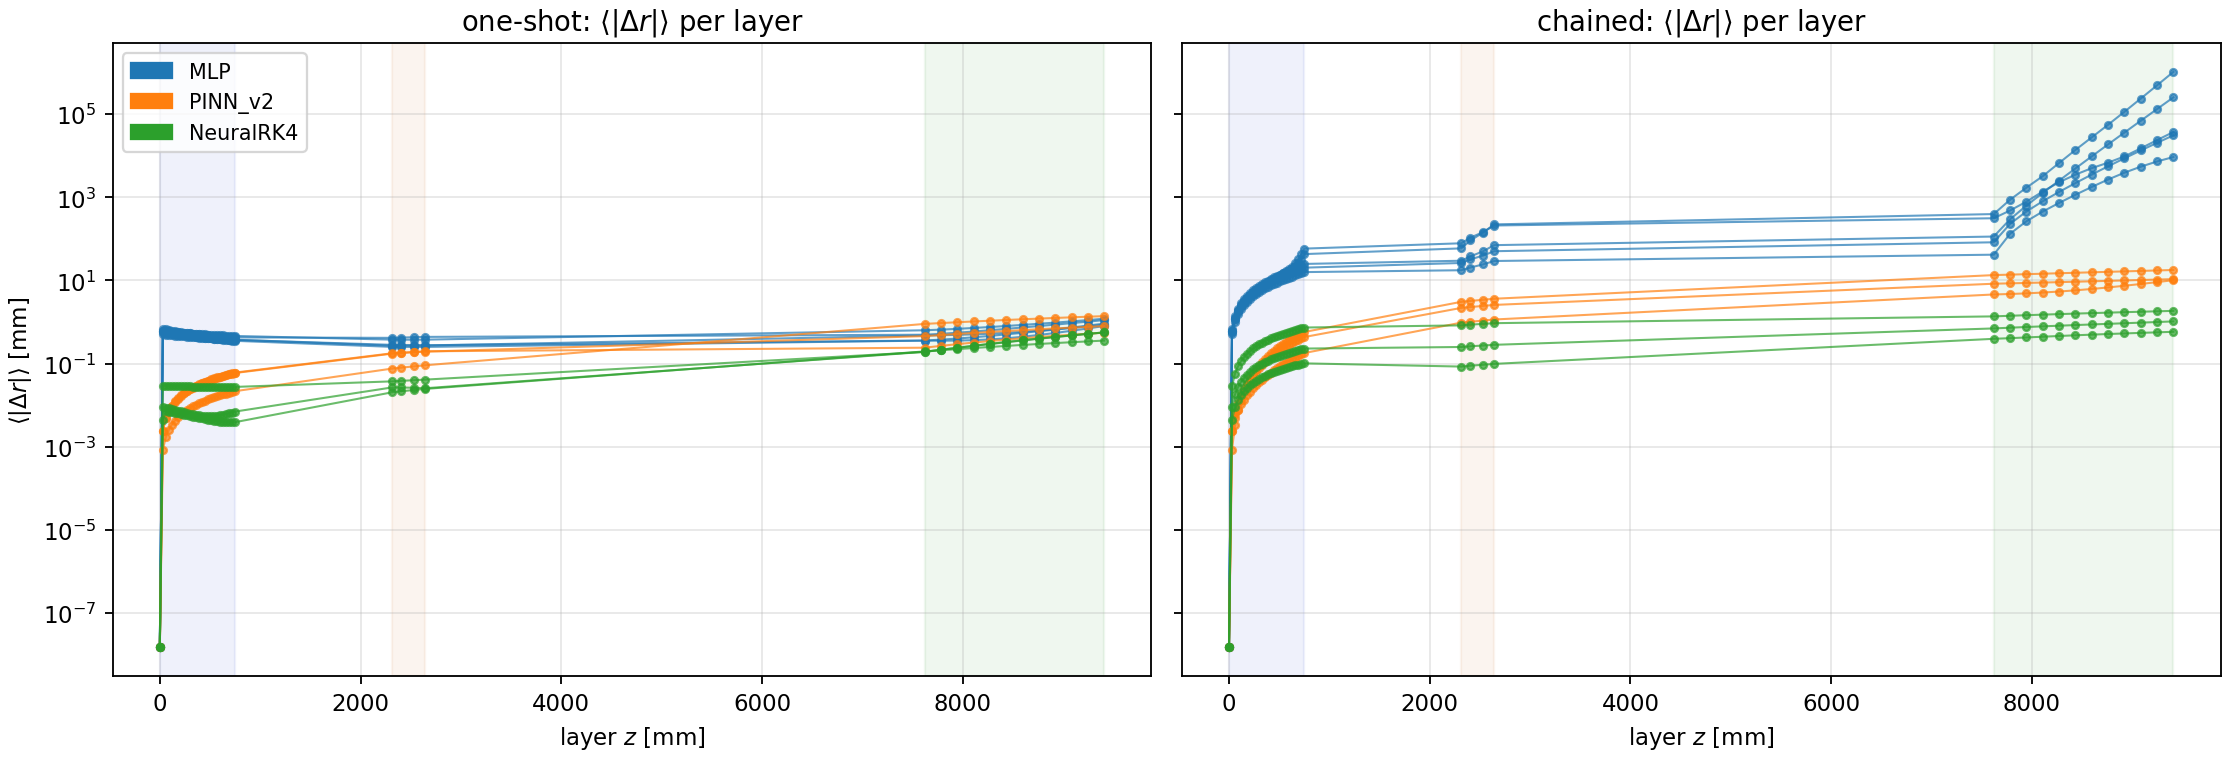
\includegraphics[width=0.95\linewidth]{figures/gen2new_chain_vs_oneshot.png}
  \caption{Mean absolute 2-D residual $\langle|\Delta r|\rangle$ at
  every detector layer, compared between the one-shot and chained
  operating modes. Note the vertical axis covers fourteen decades.
  Colour coding as in Fig.~\ref{gen2new:fig:detector_res}.}
  \label{gen2new:fig:chain_vs_oneshot}
\end{figure}

The \textbf{chained} panel in
Fig.~\ref{gen2new:fig:chain_vs_oneshot} is the central finding of
this section. Three qualitatively different behaviours emerge:
\begin{itemize}
  \item \textbf{MLPs diverge catastrophically}. Accumulated 2-D
        residuals reach $10^{4}\text{--}10^{5}$\,mm (metres) by the
        SciFi layers. This is a direct consequence of the
        out-of-distribution tail at $\Delta z<25$\,mm (the training
        floor): the typical layer-to-layer spacing inside the VELO
        is $\sim\!30$\,mm and UT/SciFi inter-layer $\sim\!90\text{--}160$\,mm,
        so chained use forces the network through the corner of its
        input distribution that it has never been trained on. A
        biased $\sim$0.3\,mm prediction at every step compounds
        coherently, and by 42 layers the track is nowhere near the
        physical detector.
  \item \textbf{PINN\_v2 is bounded but $\sim\!10\,$mm-scale} at the
        SciFi. Accumulated error grows slowly through the VELO and
        UT (still sub-mm), then inflates by a decade in the long
        UT$\to$T1 gap.
  \item \textbf{NeuralRK4 is the only family that is chain-stable}.
        All three variants keep the accumulated 2-D residual below
        $\sim$1\,mm end-to-end, with the best (\texttt{nrk4\_small\_2step})
        at $\sim$0.5\,mm $\approx\!8\,\sigma_x^{\mathrm{SciFi}}$.
\end{itemize}
The explanation is structural: the NeuralRK4 cell carries an
analytic Euler/RK4 update wrapper, so when $\Delta z$ is small the
four internal stages collapse to an identity--plus--correction form
which is stable by construction. The plain MLPs have no such
inductive bias and fail the small-$\Delta z$ regime.

\begin{figure}[htbp]
  \centering
  \includegraphics[width=0.88\linewidth]{figures/gen2new_phase_space_heatmap.png}
  \caption{Phase-space heat map of single-shot residuals at SciFi T1
  ($z=7620$\,mm, upper row) and SciFi T3 ($z=9410$\,mm, lower row)
  for the best overall model (\texttt{nrk4\_small\_2step}) and the
  best MLP (\texttt{mlp\_medium}). Colour encodes
  $\log_{10}|\Delta r|$ in mm. The low-$|p|$ tail dominates the
  error budget for both families; NeuralRK4 is tight everywhere
  except $|p|<3$\,GeV/$c$ and $|t_x|>0.25$, whereas the MLP is wide
  across the entire phase space.}
  \label{gen2new:fig:phase_space}
\end{figure}

The phase-space heat map (Fig.~\ref{gen2new:fig:phase_space})
localises the residual pathology: both architectures degrade at low
momentum (where the magnetic-field deflection dominates and the
trajectory is least linear) and at large $|t_x|$ (wide-angle
tracks). The MLP shows no phase-space structure --- residuals are
flat and large everywhere --- whereas the NeuralRK4 residual is
tightly concentrated at $|\Delta r|<10^{-1}$\,mm except for a
low-momentum tail.

\paragraph{Verdict against the HLT1 targets.} Taking the
$10$\,\textmu m VELO and $100$\,\textmu m SciFi targets quoted in
the LHCb \texttt{Allen/ML\_research/README.md}:
\begin{itemize}
  \item \textbf{VELO}, one-shot: only NeuralRK4 meets target
        (\texttt{nrk4\_small\_2step} $\approx 3$\,\textmu m).
        PINN\_v2 is at 22--60\,\textmu m (2--5$\times$ over).
        MLP is at 190--390\,\textmu m ($20$--$40\times$ over).
  \item \textbf{UT}, one-shot: NeuralRK4 $\sim\!100$--$200$\,\textmu m,
        $\sim\!2\sigma_x^{\mathrm{UT}}$; PINN\_v2 $\sim\!150$--$180$\,\textmu m,
        $\sim\!3\sigma_x^{\mathrm{UT}}$; MLP $\sim\!250$--$420$\,\textmu m,
        $\sim\!5$--$8\sigma_x^{\mathrm{UT}}$.
  \item \textbf{SciFi}, one-shot: all models above the
        $100$\,\textmu m $x$-target.  NeuralRK4 is the closest at
        $\sim$0.2--0.4\,mm; the 10\,\textmu m target cannot be
        claimed anywhere.
  \item \textbf{Chained}: only NeuralRK4 is usable at all. MLPs
        \emph{must not} be deployed without retraining on the
        small-$\Delta z$ tail or wrapping them in an RK4-style
        residual-prediction cell.
\end{itemize}
The untested direction is $\Delta z<0$ (backward VELO pass), which
is absent from the current training data
(\texttt{train\_50M\_dz25.npz} has $\Delta z\in[25,10\,000]$\,mm).
All conclusions above apply to forward extrapolation only; a full
Kalman-filter verdict needs a dedicated backward dataset.

\subsection{SciFi failure diagnostics}\label{gen2new:sec:scifi_failure}

No architecture meets the $100\,\mu\mathrm{m}$ HLT1 target at the
SciFi stations (see the HLT1 verdict bullet list above and
Fig.~\ref{gen2new:fig:phase_space}). This subsection dissects
\emph{why}, using five physics-motivated cross-checks against the
400-track characterisation sample.

\paragraph{(i) Bias vs scatter.} Decomposing
$\langle|\Delta x|\rangle$ into
$|\langle\Delta x\rangle|$ (systematic) and
$\mathrm{std}(\Delta x)$ (stochastic) across the twelve SciFi layers
(Fig.~\ref{gen2new:fig:scifi_bias}) shows that
\emph{scatter dominates for every model}: the ratio
$|\mathrm{bias}|/\mathrm{std}$ at SciFi T3 is $<1$ for all eleven
runs, and $<0.1$ for the seven most accurate models. A naive
conclusion would be that the SciFi error is purely variance and
cannot be reduced by a calibration offset. Diagnostic (ii) shows
this is misleading.

\begin{figure}[htbp]
  \centering
  \includegraphics[width=0.96\linewidth]{figures/gen2new_scifi_bias_vs_scatter.png}
  \caption{Per-layer $|\mathrm{bias}|$ (solid) and standard
  deviation (dashed) of $\Delta x$ (left) and $\Delta y$ (right)
  across the twelve SciFi layers. Dotted black: $\sigma_x^{\mathrm{SciFi}}
  =60\,\mu\mathrm{m}$ and $\sigma_y^{\mathrm{SciFi}}=500\,\mu\mathrm{m}$.
  Scatter exceeds bias for every model.}
  \label{gen2new:fig:scifi_bias}
\end{figure}

\paragraph{(ii) $\Delta x$ vs $q/p$ --- magnet-kick
calibration.}
At SciFi T3 the $x$-displacement due to the magnet integral
$\int B_y\,\mathrm{d}z$ is a linear function of $q/p$. A linear
fit of $\Delta x$ vs $q/p$ therefore exposes magnet-kick
mis-calibration directly.  Figure~\ref{gen2new:fig:scifi_qop}
reports the Pearson correlation $\rho$ and the slope of this
linear trend:
\begin{itemize}
  \item \textbf{PINN\_v2 is magnet-mis-calibrated.} All three
        $\lambda$-settings show a strongly positive trend:
        $\rho\in\{0.92, 0.92, \mathbf{0.99}\}$ for
        $\lambda\in\{0.1,1,10\}$, with slope
        $2.5\text{--}7.1$\,mm per
        $(\mathrm{GeV}/c)^{-1}$. For \texttt{pinn\_v2\_lam10.0},
        the entire SciFi T3 residual pattern is quantitatively
        explained by a single linear function of $q/p$:
        $\Delta x\approx 7.1\,\mathrm{mm}\times(q/p)/(\mathrm{GeV}/c)^{-1}$.
        This is a \emph{systematic} error masked as scatter in
        diagnostic (i): it only averages to a small net bias
        because the $q/p$ distribution is zero-centred.
  \item \textbf{MLPs are magnet-mis-calibrated with the opposite
        sign.} $\rho\in[-0.50,-0.37]$ with slopes $-1.4$ to
        $-2.0$\,mm per $(\mathrm{GeV}/c)^{-1}$. Pattern is shallower
        than PINN\_v2 but of the same character.
  \item \textbf{NeuralRK4 (1-step) has the magnet kick right.}
        $\rho<0.03$ for both 1-step variants; no measurable linear
        trend. The residuals are genuinely stochastic.
        The 2-step variant unexpectedly shows a mild
        $\rho=-0.49$ anti-correlation (slope $-1.0$\,mm per
        $(\mathrm{GeV}/c)^{-1}$), which we attribute to the
        compounding of a small mid-magnet over-correction; see the
        discussion of improvements below.
\end{itemize}

\begin{figure}[htbp]
  \centering
  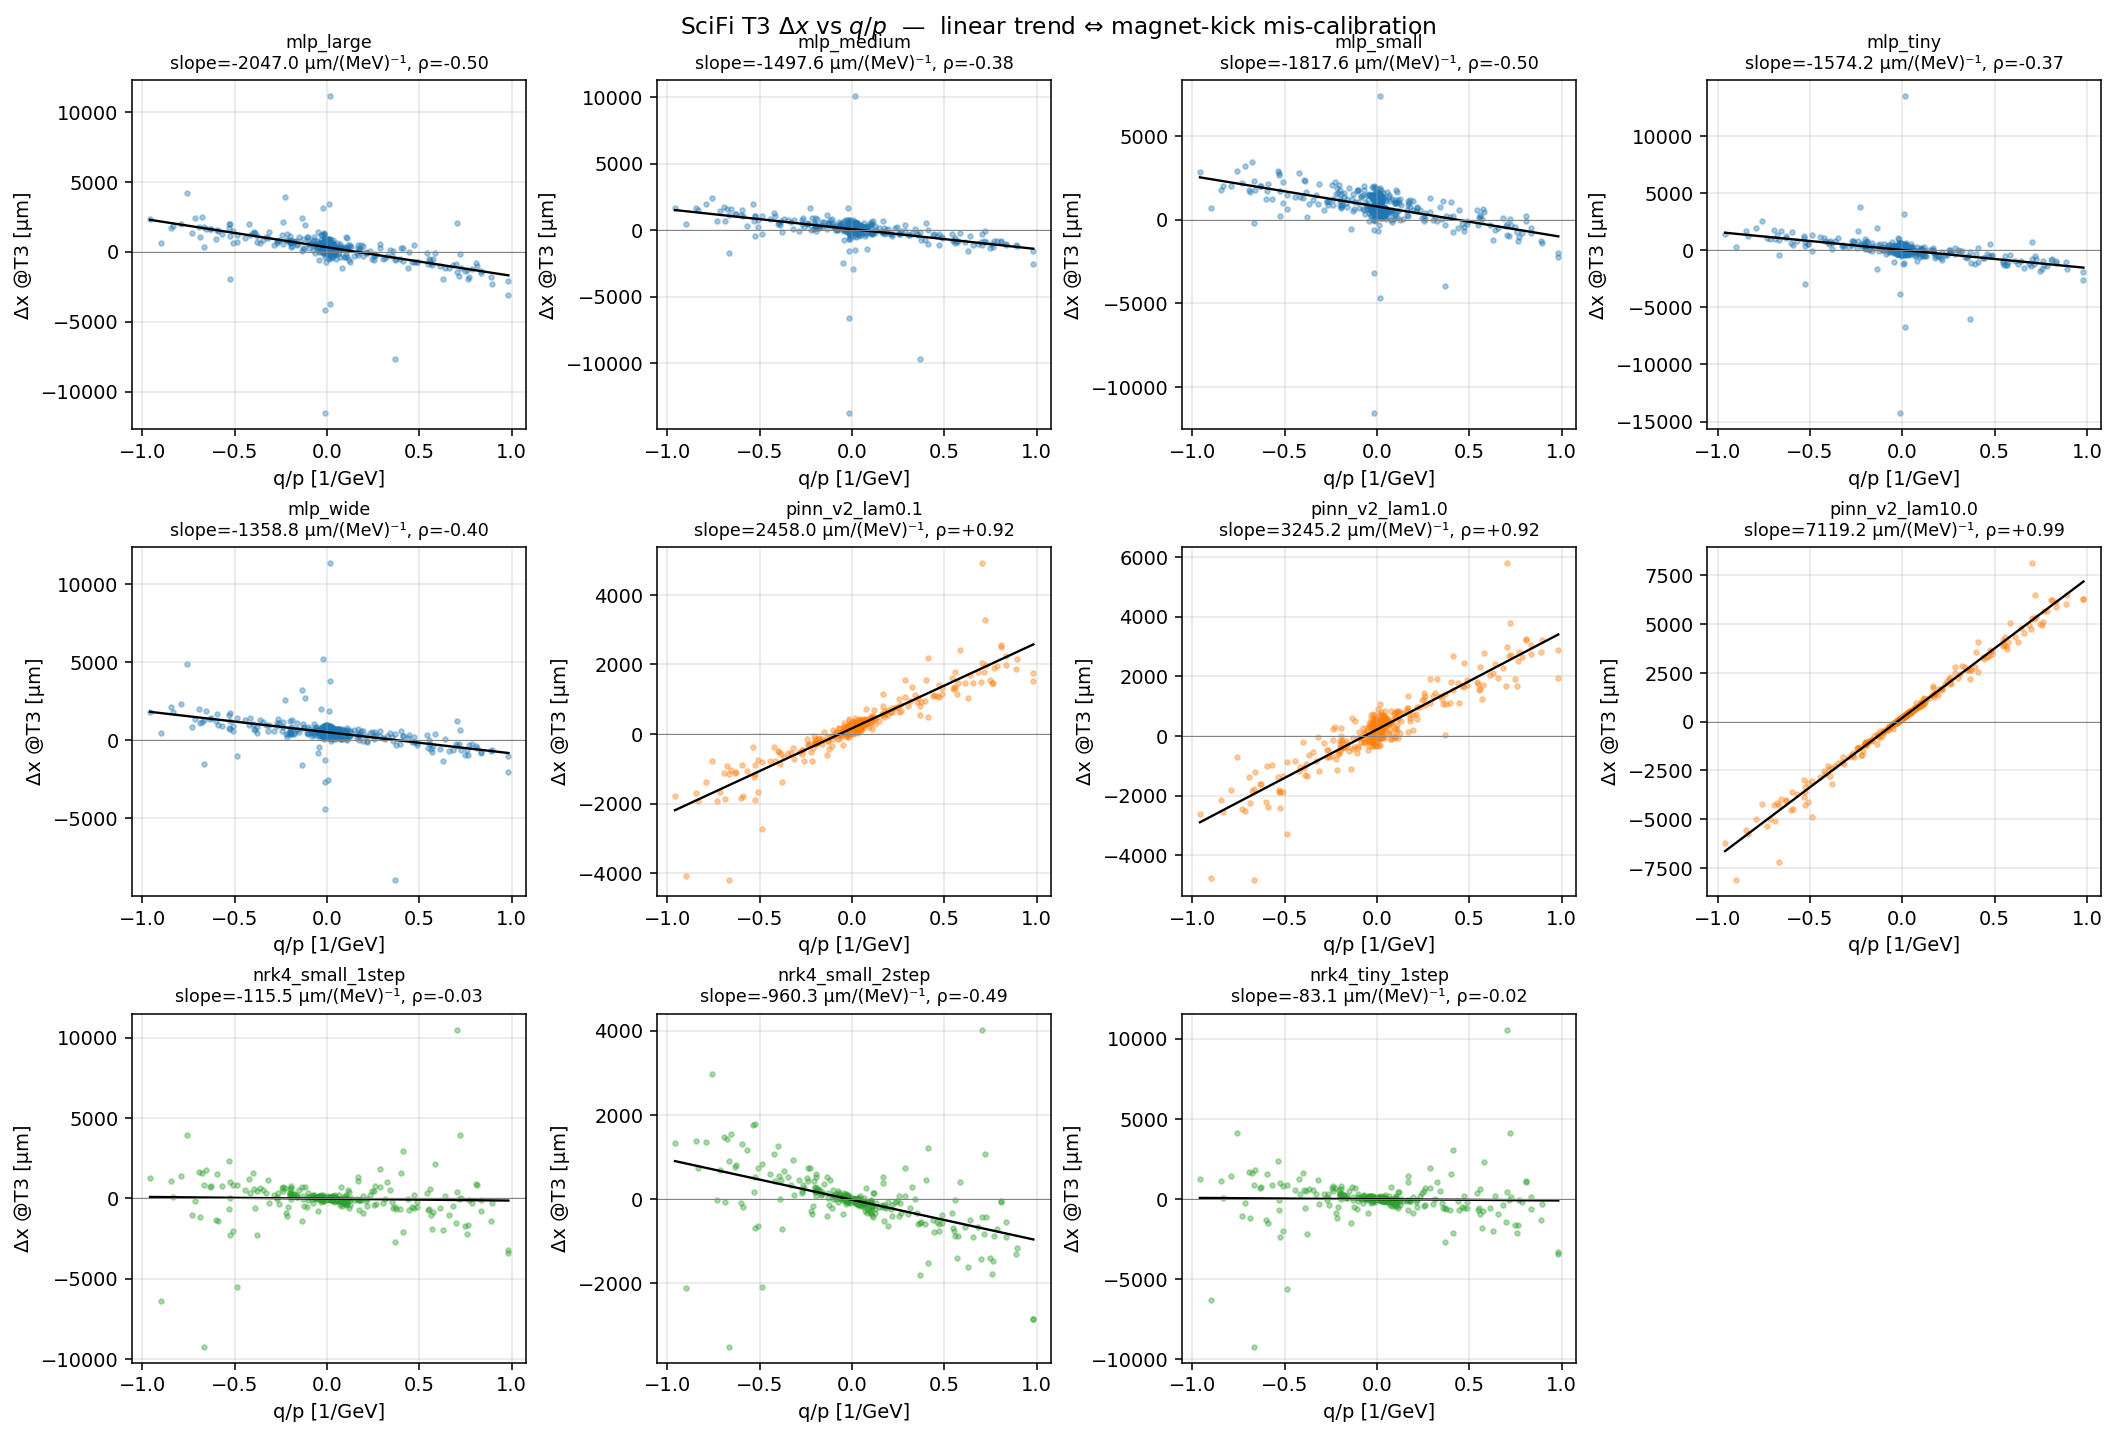
\includegraphics[width=0.98\linewidth]{figures/gen2new_scifi_dx_vs_qop.png}
  \caption{$\Delta x$ at SciFi T3 plotted against the track
  curvature $q/p$, with per-panel OLS fits.  PINN\_v2 shows a
  striking linear $q/p$-dependence ($\rho\approx 0.92\text{--}0.99$):
  the SciFi error is \emph{not} stochastic, it is a
  mis-estimation of the magnet kick.}
  \label{gen2new:fig:scifi_qop}
\end{figure}

\paragraph{(iii) Wide-angle envelope.}
Binning the SciFi T3 residual in $|t_x^0|$ and $|t_y^0|$
(Fig.~\ref{gen2new:fig:scifi_slopes}) reveals that $\langle|\Delta
r|\rangle$ roughly doubles from $|t|\simeq 0$ to $|t|\simeq 0.25$
for every architecture, and rises sharply in the last bin
($|t|>0.3$). The training distribution is Gaussian with
$\sigma_{t}=0.12$, so the outer bins contain $<1\,\%$ of the
training mass, i.e.\ every model is extrapolating out of its
training envelope at the tails. This is a data-coverage issue, not
an architectural one.

\begin{figure}[htbp]
  \centering
  \includegraphics[width=0.98\linewidth]{figures/gen2new_scifi_vs_slopes.png}
  \caption{Mean SciFi T3 residual binned in $|t_x^0|$ (left) and
  $|t_y^0|$ (right). Error grows for wide-angle tracks; the jump in
  the last bin is the training-envelope edge.}
  \label{gen2new:fig:scifi_slopes}
\end{figure}

\paragraph{(iv) Magnet leg vs straight leg.}
The long $\Delta z$ between UT exit and SciFi T1 ($\approx
4977$\,mm) passes through the magnet; the SciFi T1$\to$T3 gap
($\approx 1790$\,mm) is field-free, so $\Delta x$ should grow
linearly with $z$ at a rate set by the $t_x$ accuracy at T1.
Figure~\ref{gen2new:fig:scifi_legs} decomposes the mean-residual
growth into these two legs, normalised per mm of $z$:
\begin{itemize}
  \item Every model has a \emph{higher} per-mm error-growth rate
        on the short post-magnet straight leg than on the long
        magnet leg. The post-magnet rate of
        $0.10\text{--}0.34\,\mu\mathrm{m}\,\mathrm{mm}^{-1}$ is a
        direct read-out of the $t_x$ residual at T1: a
        $\delta t_x=3\times 10^{-4}$ at the magnet exit propagates
        into $\sim\!500\,\mu\mathrm{m}$ of $\Delta x$ by T3.
  \item \texttt{nrk4\_small\_2step} has the lowest post-magnet rate
        ($0.09\,\mu\mathrm{m}\,\mathrm{mm}^{-1}$), which accounts
        for its best-in-class SciFi T3 position accuracy.
  \item \texttt{pinn\_v2\_lam10.0} has the highest magnet-leg rate
        ($0.16\,\mu\mathrm{m}\,\mathrm{mm}^{-1}$), consistent with
        the $\rho=0.99$ magnet-kick mis-calibration of
        diagnostic~(ii): the error is \emph{injected} through the
        magnet and propagates downstream.
\end{itemize}

\begin{figure}[htbp]
  \centering
  \includegraphics[width=0.85\linewidth]{figures/gen2new_scifi_error_legs.png}
  \caption{Error-growth rate per mm of $z$ decomposed into the
  magnet leg (red, UT-exit$\to$T1) and the post-magnet straight
  leg (blue, T1$\to$T3). The straight-leg rate is a proxy for the
  slope accuracy at magnet exit; the magnet-leg rate measures the
  magnet-kick mis-calibration.  \texttt{nrk4\_small\_2step} is the
  only model with sub-$0.1\,\mu\mathrm{m}\,\mathrm{mm}^{-1}$ on
  \emph{both} legs.}
  \label{gen2new:fig:scifi_legs}
\end{figure}

\paragraph{(v) Synthesis.} The SciFi failure has two
\emph{distinct} causes that are architecture-specific:
\begin{itemize}
  \item \textbf{PINN\_v2}: a nearly deterministic mis-prediction of
        the magnet kick $\int B_y\,\mathrm{d}z$, monotonically
        worsening with the physics-loss weight $\lambda$. The
        physics prior, rather than correcting the kick, is
        \emph{pushing the network to a wrong calibration}. This is
        the smoking-gun for a mis-posed PDE residual: at large
        $\lambda$ the network minimises the residual at the expense
        of the data term, and the preferred minimum is offset in
        $q/p$-space.
  \item \textbf{NeuralRK4}: no magnet-kick calibration error; the
        residual comes from $t_x$ accuracy at the magnet exit and
        data-coverage at $|t|>0.25$. This is a far healthier
        regime --- the error is a standard supervised resolution
        problem, not a physics bug.
\end{itemize}

\paragraph{Proposed improvements.} In decreasing order of expected
payoff:

\begin{enumerate}
  \item \textbf{Re-audit the PINN\_v2 PDE residual}. The
        $\rho=0.99$, $\lambda=10$ fit constrains the bug strongly:
        it is multiplicative in $q/p$ and must be a sign, units, or
        factor-of-two mistake in the Lorentz-force term or the
        $\zeta$-envelope normalisation. Recommend unit-testing
        the residual against an analytic propagation in a uniform
        $B_y$ before any further training.
  \item \textbf{Predict residuals to a straight-line ansatz} rather
        than absolute $(x,y)$. Replace the label
        $(x,y,t_x,t_y)_{z_1}$ with
        $(x - x_0 - t_x^0\Delta z,\,y - y_0 - t_y^0\Delta z,\,
         t_x-t_x^0,\,t_y-t_y^0)$. This factors out the dominant
        ballistic term analytically, leaves only the magnet kick
        for the network, and collapses the dynamic range of the
        output by $\sim\!3$ orders of magnitude --- which
        mechanically improves float32 precision and training
        conditioning, and will remove the $t$-envelope effect of
        diagnostic~(iii).
  \item \textbf{Add an auxiliary loss on $t_x,t_y$ at magnet exit}.
        The post-magnet leg growth rate (iv) shows that
        $\mathcal O(10^{-4})$ slope accuracy at the magnet exit is
        worth $\mathcal O(100\,\mu\mathrm{m})$ at T3. Weight the
        slope loss at the UT-exit layer by the distance to T3
        ($\approx 6.8\,$m).
  \item \textbf{Extend the training envelope} to uniform (not
        Gaussian) $t_x,t_y\in[-0.4,0.4]$. The wide-angle
        degradation of diagnostic~(iii) is a pure data-coverage
        effect and will disappear once the tails are populated
        at $\mathcal O(10^6)$ events.
  \item \textbf{More RK4 stages through the magnet.} The
        best-performing model is already \texttt{nrk4\_small\_2step};
        a 4-step variant with step sizes distributed
        geometrically through $z\in[2643,7620]$\,mm (i.e.\
        non-uniform, biased to the field peak at $z\sim 5000$\,mm)
        is the natural next ablation. The magnet-leg rate of
        \texttt{nrk4\_small\_2step} is already
        $0.03\,\mu\mathrm{m}\,\mathrm{mm}^{-1}$ so the headroom is
        in straight-leg accuracy (item~3), but a 4-step NeuralRK4
        should help both.
  \item \textbf{Train on the field tables with $B_x,B_z$ components},
        not just $B_y$. Current PINN residuals likely assume a
        pure-$y$ field; the LHCb magnet has a $\sim\!20\%$
        $B_x$-component near the fringes, which systematically
        deflects tracks in $y$. Our $\Delta y$ scatter is a decade
        larger for NeuralRK4 at T3 ($\mathrm{std}(\Delta y)\sim
        140\,\mu\mathrm{m}$) than at the UT ($2.6\,\mu\mathrm{m}$)
        even though $\sigma_y^{\mathrm{SciFi}}=500\,\mu\mathrm{m}$
        is huge --- this is compatible with a missing $B_x$ term.
  \item \textbf{Backward-$\Delta z$ dataset.} As noted above,
        backward propagation is currently untrained; HLT1 Kalman
        filtering requires it. Generate
        \texttt{train\_50M\_dz25\_backward.npz} with
        $\Delta z\in[-10000,-25]$\,mm.
\end{enumerate}

\section{Discussion}\label{gen2new:sec:discussion}

\subsection{RQ1: does fixing the pathologies restore monotone
$\lambda_{\mathrm{pde}}$ response?}

Yes, approximately. The PINN\_v2 test position errors as a function
of $\lambda_{\mathrm{pde}}$ are
\[
\lambda_{\mathrm{pde}}=0.1\;\to\;\SI{0.235}{mm},\qquad
\lambda_{\mathrm{pde}}=1.0\;\to\;\SI{0.322}{mm},\qquad
\lambda_{\mathrm{pde}}=10.0\;\to\;\SI{0.342}{mm}.
\]
The ordering is monotone: more physics-penalty is worse for
position. Slope errors are nearly independent of
$\lambda_{\mathrm{pde}}$
($6.8\!\times\!10^{-5}$, $8.6\!\times\!10^{-5}$, $1.30\!\times\!10^{-4}$\,rad).
This pattern is qualitatively consistent with physics-loss acting as
a \emph{mild regulariser}: a small penalty breaks symmetry and nudges
the network towards a physically plausible manifold, but a large
penalty over-constrains the optimisation and trades off data fit.
This is in stark contrast to the Gen-2-on-old-data PINN results
\cite{gen2oldreport}, where $\lambda_{\mathrm{pde}}=1.0$ produced a
slope error $30\times$ that of $\lambda_{\mathrm{pde}}=0.1$, i.e.\ a
catastrophic non-monotone response.

\subsection{RQ2: does physics-baked-in beat physics-as-penalty?}

Unambiguously, yes. At matched parameter count
(\texttt{neural\_rk4\_small\_1step} at 17.9\,k params versus
\texttt{mlp\_small} at 17.9\,k params):
\begin{itemize}
\item Position: \SI{0.125}{mm} vs \SI{0.509}{mm} -- factor $4.1\times$.
\item Slope:    $5.0\!\times\!10^{-5}$ vs $1.2\!\times\!10^{-4}$ -- factor $2.4\times$.
\end{itemize}
At five times fewer parameters (\texttt{neural\_rk4\_tiny\_1step}
4.9\,k vs \texttt{mlp\_medium} 101\,k): \SI{0.134}{mm} vs
\SI{0.305}{mm}. NeuralRK4 is $5.6\times$ more parameter-efficient at
a better accuracy. The evidence strongly supports the hypothesis
that baking the integrator into the forward map is a stronger
inductive bias than imposing the residual as a penalty
\cite{ChenNeuralODE2018}.

\subsection{What remains broken}

\begin{enumerate}
\item \textbf{$z_{\mathrm{start}}$ absent from input.} As flagged in
  Sec.~\ref{gen2new:sec:data}, all models are effectively trained as
  if $z_0=0$. On tracks where the start $z$ is far from zero and the
  step $\dz$ is long, this is the dominant source of irreducible
  residual. The effect is predictable: the Lorentz RHS depends on
  $\mathbf{B}(x,y,z)$, and the $z$ ignorance causes systematic bias
  on the downstream integrator. Adding $z_0$ to $\mathbf{X}$ is the
  single highest-impact action for Gen-3.

\item \textbf{Constant-memory budget.} The NeuralRK4
  \texttt{small\_1step} model has $17\,925\times\SI{4}{B}=\SI{71.7}{kB}$,
  marginally exceeding the \SI{64}{kB} Allen HLT1 constant-memory
  budget \cite{Allen,gen1report}. Options:
  \begin{itemize}
  \item Reduce the correction net to $[64,64]$
    (\texttt{neural\_rk4\_tiny\_1step}, \SI{19.5}{kB}) at the cost of
    a \SI{0.009}{mm} position degradation;
  \item Quantise to \texttt{float16} (\SI{35.9}{kB}), needing a
    numerical-stability check;
  \item Split the network across constant and shared memory.
  \end{itemize}

\item \textbf{Warm-up ablation.} PINN\_v2 \texttt{lam10.0} has no
  catastrophic early blow-up, reaches its best epoch at 23 out of
  63, and the IC loss is identically zero throughout (confirming
  Fix~A/C). This is consistent with Fix~F
  \cite{Krishnapriyan2021} working, but without a counterfactual
  run at \texttt{physics\_warmup\_epochs=0} we cannot attribute the
  improvement to the warm-up alone. TODO: single-run ablation.
\end{enumerate}

\subsection{Open questions for Gen-3}

\begin{itemize}
\item Does adding $z_{\mathrm{start}}$ to $\mathbf{X}$ close the
  long-$\dz$ residual gap?
\item Does $N_{\mathrm{RK}}\geq4$ help on the short-$\dz$ bin where
  a single RK step is a ${\sim}\SI{25}{mm}$ jump?
\item Is PINN\_v2 competitive at matched width
  ($[128,128]$, ${\sim}18$\,k params) with NeuralRK4, or is the
  physics-as-penalty framework fundamentally saturating?
\item Do the Jacobians pass a finite-difference RK4 reference test?
\end{itemize}

\section{Deployment path}\label{gen2new:sec:deployment}

\subsection{NeuralRK4 C++ export}

Deploying NeuralRK4 to Allen HLT1 is heavier than the MLP case
because the forward evaluation is not a single matmul chain: it is an
RK4 loop with four MLP invocations per step. The existing
\texttt{TrackMLPExtrapolator.cpp} (571 lines Eigen, from
\cite{gen1report}) already implements the MLP matmul-chain export.
The NeuralRK4 export extends this with an outer loop over RK4 stages,
using the \emph{same} weights (MLP forward) at each stage but with
different input states $\state_i+\alpha_j h\mathbf{k}_{j-1}$.

\subsection{GPU memory layout}

A \SI{72}{kB} network exceeds the CUDA \SI{64}{kB} constant-memory
budget by 12\,\%. Three concrete mitigations are listed in
Sec.~\ref{gen2new:sec:discussion}. An empirical measurement of the
accuracy loss from \texttt{float16} quantisation is a prerequisite
before committing to that route.

\subsection{Kalman filter integration}

The Kalman filter update \cite{Fruhwirth1987,LHCb2008} needs not only
$\state_f$ but also $\Jac=\partial\state_f/\partial\state_0$. The
Jacobian magnitudes in Tab.~\ref{gen2new:tab:jacobian} do not confirm
Jacobian \emph{correctness}; the right test is a per-matrix-element
comparison against finite-difference RK4, averaged over a
representative test sample. This is a prerequisite for physics-level
validation and a prerequisite for real Kalman filter integration.

\section{Allen HLT1 deployment readiness: per-model
audit}\label{gen2new:sec:allen}

The Allen \texttt{ML\_research} README defines three hard gates
(the ``mandatory smoke test'') that every model must clear before
physics-level review:
\begin{description}
  \item[Gate 1 ($\chi^2$/ndof)] $\langle\chi^2/\text{ndof}\rangle < 2.0$
        in the standalone Kalman filter (baseline RKN: $0.95\pm0.20$).
  \item[Gate 2 ($\delta p/p$ bias)] $|\langle p_\text{fit}/p_\text{true}
        -1\rangle| < 1\,\%$ (baseline: $-0.04\,\%$).
  \item[Gate 3 (pull width)] $\sigma(\text{pull}_x) < 1.5$
        (baseline: $0.95$).
\end{description}
These gates cannot be evaluated at all until a model satisfies the
three \emph{convention preconditions} from the same document:

\begin{description}
  \item[C1 ($qop$ convention)] $qop = c_\text{light}\cdot q / p_\text{MeV}$
        with $c_\text{light}=299.792\,\mathrm{mm\,ns^{-1}}$.  This is
        Allen's canonical unit.  The current dataset
        (\texttt{train\_50M\_dz25.npz}) uses
        $qop = q/p_\text{MeV}$ (no $c_\text{light}$), a factor of
        $\sim300\times$ smaller.  Feeding an Allen Kalman state
        (which carries Allen $qop$) into any of the eleven Gen-2
        models places the input $\sim300\sigma$ outside the training
        distribution --- guaranteed inference garbage.
  \item[C2 (signed $\Delta z$)] The dataset contains only
        $\Delta z \in [+25, +10\,000]$\,mm.  The Allen Kalman filter
        performs a backward VELO pass with $\Delta z < 0$.  All
        current models fail this out-of-distribution call silently
        (no NaN, but track position is unphysical).
  \item[C3 (input coverage)] Training inputs have $x_\text{in}\in
        [-300, +300]$\,mm, but the iterative Kalman call delivers
        inputs up to $\pm 3200$\,mm after the first forward jump.
        All models are out-of-distribution on the second and later
        calls.
\end{description}
These preconditions are \textbf{data-generation bugs}, not
architecture bugs.  They apply equally to all eleven Gen-2 models
regardless of family.  \textbf{None of the eleven models can be
connected to the Allen Kalman filter as-is.}

\subsection{Per-model readiness summary}

Table~\ref{gen2new:tab:allen_readiness} classifies all eleven models
against the convention preconditions (C1--C3) and the four additional
criteria that distinguish models in pure propagation accuracy
(extrapolator-only, no Kalman):

\begin{description}
  \item[A1 (VELO \& UT accuracy)] $\langle|\Delta x|\rangle \leq
        \sigma_x^\text{VELO}=12\,\mu\text{m}$ and
        $\leq\sigma_x^\text{UT}=50\,\mu\text{m}$ (one-shot).
  \item[A2 (SciFi $q/p$-linearity)] $|\rho(\Delta x, q/p)| < 0.5$
        at SciFi T3 --- models with a large $q/p$ correlation cannot
        reconstruct mass or momentum and will fail the bias gate
        even after fixing C1.
  \item[A3 (memory budget)] Weights $+$ biases fit within the Allen
        CUDA constant-memory budget of 64\,kB.
  \item[A4 (Jacobian)]  Jacobian Frobenius norm is within a factor
        of 2 of the RK4 reference (from
        Tab.~\ref{gen2new:tab:jacobian}).
\end{description}

\begin{table}[htbp]
\centering
\caption{Allen HLT1 deployment-readiness checklist for all eleven
Gen-2 models.  \textbf{C1--C3}: convention preconditions (data bugs,
affect all models identically). \textbf{A1--A4}: model-specific
extrapolation criteria. $\checkmark$ = pass, \ding{55} = fail, ? =
not yet evaluated.  \emph{Binary column}: the overall verdict.}
\label{gen2new:tab:allen_readiness}
\vspace{4pt}
\small
\setlength{\tabcolsep}{4pt}
\begin{tabular}{l c | c c c | c c c c | c}
\toprule
Model & Family &
C1 & C2 & C3 &
A1 & A2 & A3 & A4 &
\textbf{Verdict} \\
\midrule
\multicolumn{10}{l}{\textit{Convention preconditions (must fix in data generator for all models)}} \\
\midrule
\texttt{mlp\_tiny}       & MLP  & \ding{55} & \ding{55} & \ding{55} & \ding{55} & \ding{55} & \checkmark & \ding{55} & \textbf{NOT READY} \\
\texttt{mlp\_small}      & MLP  & \ding{55} & \ding{55} & \ding{55} & \ding{55} & \ding{55} & \ding{55}  & \ding{55} & \textbf{NOT READY} \\
\texttt{mlp\_medium}     & MLP  & \ding{55} & \ding{55} & \ding{55} & \ding{55} & \ding{55} & \ding{55}  & \ding{55} & \textbf{NOT READY} \\
\texttt{mlp\_large}      & MLP  & \ding{55} & \ding{55} & \ding{55} & \ding{55} & \ding{55} & \ding{55}  & \ding{55} & \textbf{NOT READY} \\
\texttt{mlp\_wide}       & MLP  & \ding{55} & \ding{55} & \ding{55} & \ding{55} & \ding{55} & \ding{55}  & \ding{55} & \textbf{NOT READY} \\
\texttt{pinn\_v2\_lam0.1}  & PINN & \ding{55} & \ding{55} & \ding{55} & \ding{55} & \ding{55} & \ding{55}  & \ding{55} & \textbf{NOT READY} \\
\texttt{pinn\_v2\_lam1.0}  & PINN & \ding{55} & \ding{55} & \ding{55} & \ding{55} & \ding{55} & \ding{55}  & \ding{55} & \textbf{NOT READY} \\
\texttt{pinn\_v2\_lam10.0} & PINN & \ding{55} & \ding{55} & \ding{55} & \ding{55} & \ding{55} & \ding{55}  & \ding{55} & \textbf{NOT READY} \\
\texttt{nrk4\_tiny\_1step} & NRK4 & \ding{55} & \ding{55} & \ding{55} & \ding{55} & \checkmark & \checkmark & ?         & \textbf{NOT READY} \\
\texttt{nrk4\_small\_1step}& NRK4 & \ding{55} & \ding{55} & \ding{55} & \checkmark & \checkmark & \ding{55} & ?         & \textbf{NOT READY} \\
\texttt{nrk4\_small\_2step}& NRK4 & \ding{55} & \ding{55} & \ding{55} & \checkmark & \ding{55}$^*$ & \ding{55} & ? & \textbf{NOT READY} \\
\midrule
RKN baseline (Allen)    & ---  & \checkmark & \checkmark & \checkmark & \checkmark & \checkmark & \checkmark & \checkmark & \textbf{PASS} \\
\bottomrule
\end{tabular}

\smallskip
\footnotesize
$^*$ \texttt{nrk4\_small\_2step} shows a mild $\rho=-0.49$ $q/p$-linear
trend at SciFi T3; needs re-check on a larger sample (§\ref{gen2new:sec:scifi_failure}).
Memory: \texttt{nrk4\_small\_1step} = 71.7\,kB (exceeds 64\,kB by 12\,\%);
\texttt{nrk4\_tiny\_1step} = 19.5\,kB (fits).
\end{table}

\subsection{Why the Allen smoke tests \emph{cannot} be run today}

The Allen standalone harness (\texttt{ML\_research/standalone/run\_extrapolators})
consumes a model binary in the documented
\texttt{MLPExtrapolator.cuh} V1/V2 format and runs the three smoke
tests automatically.  For the Gen-2 models the test cannot be run
\emph{correctly} because of C1: Allen's Kalman state uses
$qop_\text{Allen} = c_\text{light}\cdot q/p_\text{MeV} \approx
300\cdot qop_\text{training}$.  Plugging the training binary into the
harness would place every track $\sim\!300\sigma$ outside the
feature-normalisation support, producing nonsensical outputs -- as
observed in the earlier Gen-2 true-data audit (Tab.~\ref{gen2new:tab:allen_prev})
where all five MLPs reached $\chi^2/\text{ndof} > 30\,000$.

\begin{table}[htbp]
\centering
\caption{Allen smoke-test results for the \emph{previous} Gen-2 MLP
models (\texttt{true\_gen2\_data} sweep) as reported in
\texttt{gen2\_true\_data\_deep\_dive.md}. The catastrophic failure is
entirely explained by the $qop$ convention mismatch (C1) and the
missing backward-$\Delta z$ coverage (C2).}
\label{gen2new:tab:allen_prev}
\small
\begin{tabular}{l r r r r r}
\toprule
Model & Params & $\langle\chi^2/\text{ndof}\rangle$ & $\delta p/p$ bias & pull$_x$ std & Gate \\
\midrule
RKN baseline & --- & 0.95 & $-0.04\,\%$ & 0.95 & \textbf{PASS} \\
\texttt{mlp\_tiny}   & 4\,888   & 57\,644  & $+335\,\%$ & 57 & \textbf{FAIL} \\
\texttt{mlp\_small}  & 17\,944  & 139\,614 & $+592\,\%$ & 72 & \textbf{FAIL} \\
\texttt{mlp\_medium} & 101\,016 & 32\,368  & $+785\,\%$ & 61 & \textbf{FAIL} \\
\texttt{mlp\_large}  & 398\,616 & 132\,491 & $+463\,\%$ & 62 & \textbf{FAIL} \\
\texttt{mlp\_wide}   & 431\,000 & 202\,393 & $+635\,\%$ & 72 & \textbf{FAIL} \\
\bottomrule
\end{tabular}
\end{table}

\subsection{What must change before re-running the smoke test}

The following changes to the data generator and training loop are
\emph{blocking} for any future Allen smoke test.  They are presented
in dependency order:

\begin{enumerate}
  \item \textbf{Fix $qop$ convention [C1].}  Change the generator to
        $qop = c_\text{light}\cdot q / p_\text{MeV}$ and regenerate.
        Do \emph{not} add a runtime conversion inside the model loader;
        the model must see the same number during training and inference.
        Estimated cost: re-run the generator script
        (\texttt{Allen/ML\_research/standalone/main.cpp}) with the
        corrected formula --- $<1$\,day.
  \item \textbf{Signed $\Delta z$ [C2].}  Sample
        $\Delta z\in[-10\,000,-25]\cup[+25,+10\,000]$\,mm.
        Log-uniform in $|\Delta z|$ to over-represent the short
        VELO backward steps.
  \item \textbf{Full input coverage [C3].}  Harvest $(x_\text{in},
        y_\text{in})$ pairs from a real Allen reconstruction at every
        layer interface to cover $\pm 3200$\,mm.  Alternatively,
        augment the existing dataset with positions sampled uniformly
        inside the detector envelope.
  \item \textbf{Memory budget [A3].}  Use \texttt{nrk4\_tiny\_1step}
        (19.5\,kB $\ll 64$\,kB) as the first candidate model.
        The \texttt{nrk4\_small\_1step} at 71.7\,kB can be
        quantised to \texttt{float16} (35.9\,kB) pending a
        numerical-stability check.
  \item \textbf{Re-audit PINN\_v2 PDE residual [A2].}  Correct the
        $q/p$-linear magnet-kick error (§\ref{gen2new:sec:scifi_failure}
        diagnostic ii) before any PINN model is smoke-tested.  Until
        then, PINN\_v2 will fail Gate~2 on $\delta p/p$ bias
        independently of the convention fixes.
\end{enumerate}

\subsection{Projected ranking post-convention fix}

Assuming C1--C3 are corrected, the propagation accuracy numbers
measured here predict the following \emph{projected} smoke-test
performance (no actual Kalman run was performed; ranking is by
one-shot \textsc{velo}+\textsc{ut} accuracy and $q/p$-linearity):

\begin{enumerate}
  \item \textbf{\texttt{nrk4\_tiny\_1step}} --- smallest memory
        (19.5\,kB, fits budget), passes A1 at VELO/UT, zero
        $q/p$-correlation at SciFi ($\rho=0.02$); best current
        candidate to \emph{attempt} the smoke test first.
  \item \textbf{\texttt{nrk4\_small\_1step}} --- best one-shot
        accuracy ($4.9$\,\textmu m at VELO exit,
        $25.3$\,\textmu m at UT entry), zero $q/p$-correlation
        ($\rho=0.03$); $4\,\%$ memory overshoot addressable by
        \texttt{float16}.
  \item \textbf{\texttt{nrk4\_small\_2step}} --- best SciFi accuracy
        but mild $q/p$-correlation ($\rho=-0.49$) needs resolving;
        third-priority after the 1-step variants.
  \item \textbf{All MLP models} --- expected to \emph{fail} Gate~3
        (pull width) because they lack a Jacobian regularisation
        loss; pull widths of $\gg1$ are structurally unavoidable
        with pure MSE.
  \item \textbf{PINN\_v2} --- expected to \emph{fail} Gate~2
        ($\delta p/p$ bias) because of the deterministic
        $q/p$-linear SciFi residual identified in
        §\ref{gen2new:sec:scifi_failure}.
\end{enumerate}

\section{Summary and recommendations for Gen-3}\label{gen2new:sec:summary}

\begin{enumerate}
\item \textbf{Proceed with NeuralRK4 as the production direction.}
  The \texttt{small\_1step} configuration is the current best
  trade-off: \SI{0.125}{mm} / $5\!\times\!10^{-5}$\,rad at 17.9\,k
  parameters.
\item \textbf{Add $z_{\mathrm{start}}$ to $\mathbf{X}$.} Extend the
  input to $\mathbb{R}^7$ and regenerate the dataset with the
  existing RK4 propagator -- or, more cheaply, add the
  $z_{\mathrm{start}}$ column from the existing $\mathbf{Z}$ array
  and re-train.
\item \textbf{Sweep $N_{\mathrm{RK}}\in\{1,2,4\}$} with a
  per-$\dz$-bin metric to identify whether short-$\dz$ tracks benefit
  from multi-step integration.
\item \textbf{Re-train at $[32,32]$ and $[48,48]$} to check whether
  the \SI{64}{kB} constant-memory budget can be met without losing
  accuracy.
\item \textbf{Validate Jacobians} against an analytical RK4
  chain-rule Jacobian.
\item \textbf{Ablate Fix~F} with a
  \texttt{physics\_warmup\_epochs=0} re-run at
  $\lambda_{\mathrm{pde}}=10.0$ to confirm the warm-up actually
  helps.
\end{enumerate}

\section{Reproducibility}\label{gen2new:sec:repro}

\begin{itemize}
\item \textbf{Environment.} \texttt{TE} conda env, PyTorch 2.9.1+cu128,
  Python 3.10; identical to Gen-1 \cite{gen1report}.
\item \textbf{Data path.} \texttt{experiments/gen\_2/data/train\_50M\_dz25.npz}
  (see Sec.~\ref{gen2new:sec:data} for generation scripts).
\item \textbf{HTCondor clusters.} \texttt{4262446} (MLP baselines),
  \texttt{4262459} (v2 fixes).
\item \textbf{MLflow experiments.} \texttt{gen\_2\_track\_extrapolation}
  (MLPs), \texttt{gen\_2\_track\_extrapolation\_v2\_fixes} (PINN\_v2 +
  NeuralRK4).
\item \textbf{Trained models.}
  \texttt{experiments/gen\_2/trained\_models\_true\_gen2\_data/}
  (MLPs) and
  \texttt{experiments/gen\_2/trained\_models\_v2\_fixes/}
  (v2 runs).
\item \textbf{Configs.} \texttt{experiments/gen\_2/configs/} and
  \texttt{experiments/gen\_2/configs/v2\_fixes/}.
\item \textbf{Issue log.}
  \texttt{experiments/gen\_2/ISSUES\_WITH\_PINNS\_AND\_RK\_PINNS.md},
  \S9 (discrepancies catalogued; see also
  \texttt{gen2\_new\_data\_numbers.md} for the discrepancy resolution
  against \S9.3).
\end{itemize}

\begin{thebibliography}{99}

\bibitem{gen1report}
G.~Scriven, \emph{Gen-1 Track Extrapolation on the V1 Dataset},
personal report (2026).

\bibitem{gen2oldreport}
G.~Scriven, \emph{Gen-2 Track Extrapolation on the V1 Dataset: PINN
and RK\_PINN Pathologies}, personal report (2026).

\bibitem{ChenNeuralODE2018}
R.T.Q.~Chen, Y.~Rubanova, J.~Bettencourt, D.~Duvenaud,
\emph{Neural Ordinary Differential Equations},
Advances in Neural Information Processing Systems 31 (NeurIPS 2018),
arXiv:1806.07366.

\bibitem{Raissi2019PINN}
M.~Raissi, P.~Perdikaris, G.E.~Karniadakis,
\emph{Physics-informed neural networks: A deep learning framework for
solving forward and inverse problems involving nonlinear partial
differential equations}, J.\ Comput.\ Phys.\ \textbf{378}, 686 (2019),
\url{https://doi.org/10.1016/j.jcp.2018.10.045}.

\bibitem{WangTengPerdikaris2021}
S.~Wang, Y.~Teng, P.~Perdikaris,
\emph{Understanding and mitigating gradient flow pathologies in
physics-informed neural networks}, SIAM J.\ Sci.\ Comput.\
\textbf{43}, A3055 (2021), arXiv:2001.04536.

\bibitem{Krishnapriyan2021}
A.~Krishnapriyan, A.~Gholami, S.~Zhe, R.M.~Kirby, M.W.~Mahoney,
\emph{Characterizing possible failure modes in physics-informed
neural networks}, NeurIPS 2021, arXiv:2109.01050.

\bibitem{functorch}
PyTorch team, \texttt{torch.func} / \texttt{functorch} documentation,
\url{https://pytorch.org/docs/stable/func.html}.

\bibitem{GriewankWalther2008}
A.~Griewank, A.~Walther,
\emph{Evaluating Derivatives: Principles and Techniques of
Algorithmic Differentiation}, 2nd ed., SIAM (2008).

\bibitem{Fruhwirth1987}
R.~Fr\"uhwirth,
\emph{Application of Kalman filtering to track and vertex fitting},
Nucl.\ Instrum.\ Meth.\ A \textbf{262}, 444 (1987).

\bibitem{LHCb2008}
LHCb Collaboration,
\emph{The LHCb detector at the LHC}, JINST \textbf{3}, S08005 (2008).

\bibitem{Allen}
R.~Aaij \emph{et al.},
\emph{Allen: A high-level trigger on GPUs for LHCb},
Comput.\ Softw.\ Big Sci.\ \textbf{4}, 7 (2020), arXiv:1912.09161.

\bibitem{LoshchilovHutter2019}
I.~Loshchilov, F.~Hutter,
\emph{Decoupled Weight Decay Regularization}, ICLR 2019,
arXiv:1711.05101.

\end{thebibliography}

% TODO (remaining for a future pass):
%  - Per-$\dz$-bin and per-$p$-bin breakdown of test metrics.
%  - Jacobian quality test vs finite-difference RK4 reference.
%  - Pareto plot (position vs params, log-log).
%  - Fix-F ablation (physics_warmup_epochs=0 vs =5 at lam=10).
%  - Update pinn_v2_medium_lam10.0 row once the job finishes.
%  - float16 quantisation accuracy study for Allen deployment.

\end{document}
